\documentclass[12pt]{article}
\usepackage[utf8]{inputenc}
\usepackage{algorithm}
\usepackage{algpseudocode}
\usepackage{sigsam,amsmath,amsfonts,amssymb}
\usepackage{cite}
\usepackage{url}
\usepackage{booktabs}
\usepackage{graphicx}
\usepackage{caption}
\usepackage{tikz}
\usetikzlibrary{shapes, arrows.meta, positioning, decorations.pathreplacing}
\usepackage[colorlinks]{hyperref}
\usepackage{xcolor}
\usepackage[margin=1in]{geometry}

\setlength{\parskip}{1em}
\setlength{\parindent}{0em}
\setcounter{page}{1}

\title{Modeling Regional Infectious Disease Spread with Physics-Informed Neural Networks: A Study on COVID-19 Dynamics}
\author{Michael Ajao-olarinoye \\
    Center for Computational Science and Mathematical Modelling \\
    Coventry University \\
    \url{olarinoyem@coventry.ac.uk}}
\date{}

\begin{document}

\maketitle

\begin{abstract}
    The COVID-19 pandemic has presented numerous challenges to healthcare systems globally, particularly in managing the demand for critical resources such as mechanical ventilators. Accurate forecasting of ventilator demand is paramount to ensure effective resource allocation and preparedness. This study employs a novel approach by integrating Universal Differential Equations (UDE) within a SEIR-based epidemiological model to forecast the demand for mechanical ventilators in England using real-world COVID-19 data. Our model uniquely blends data-driven machine learning components with traditional epidemiological modeling, allowing for a nuanced understanding of disease transmission dynamics and healthcare resource utilization. Utilizing data on daily case counts, hospital admissions, and mechanical ventilator usage over time, we trained neural network components to estimate key parameters dynamically. Our results indicate that the UDE-based model provides robust short-term forecasts of ventilator demand, aiding in timely resource allocation and policy interventions. This approach showcases the potential of hybrid modeling techniques in enhancing healthcare system preparedness and response during public health crises.
\end{abstract}

\section{Introduction}

The virus SARS-COV-2 causes COVID-19, a severe respiratory disease with a high mortality rate that has triggered a global pandemic \cite{forman202012}. The disease have affected more than 210 countries and territories, infecting hundreds of millions of people and killing millions. COVID-19 poses a complex and unprecedented challenge for public health and society, requiring scientific efforts to understand, model, diagnose and control the virus and disease. The COVID-19 pandemic has strained healthcare systems worldwide, requiring effective resource allocation and intervention strategies to mitigate the virus's impact \cite{emanuel2020fair}. Resource allocation is the process of distributing and allocating resources, which can include financial and non-financial assets, to achieve specific objectives or goals \cite{jiang2019emergency}. Resource allocation interventions for the COVID-19 pandemic can be divided into pharmaceutical and non-pharmaceutical interventions \cite{ehmann2021operational}. For instance, in healthcare systems, resource allocation may include both pharmaceutical resources, such as medications and vaccines, and non-pharmaceutical resources, such as ICU beds, medical equipment and personnel, to ensure effective and efficient delivery of healthcare services \cite{zaric2001resource, brandeau2004allocating}. Current studies often focus on the allocation of a single type of resource, such as pharmaceutical or non-pharmaceutical resources. However, in reality, resource allocation often involves multiple types of resources that are interrelated and have different allocation principles. Epidemiological modelling and resource demand forecasting are essential for informing resource allocation decisions. These models use data on various factors, such as disease prevalence, population demographics, and healthcare capacity, to predict the demand for different types of resources.

These will help in developing strategies for disease prevention and control, as well as sustainable public health policies and economic activity guidelines. Mathematical models have always been useful in understanding the transmission mechanisms of a disease outbreak and providing valuable insights for controlling it. 

There are different ways to model infectious diseases like covid-19. One way is to count the number of people who are infected, recovered, dead, or susceptible in an epidemic. This is called the compartmental model, and it is the most popular mathematical model that researchers use to study the disease. The compartmental model can be either deterministic or stochastic. Deterministic models can simulate a general scenario of how the disease spreads. Stochastic models can simulate how the disease spreads in small or sub-grouped populations, or predict the possible outcomes. Other mathematical models have also been used to describe infectious disease, such as in

\section{Literature Review}

The literature on COVID-19 has rapidly expanded since the onset of the pandemic, covering various aspects from epidemiological modeling to healthcare resource allocation. Key studies have focused on the development and application of compartmental models, such as the SIR and SEIRD models, to predict the spread of COVID-19 and its impact on public health systems. Recent advancements in machine learning, particularly Physics-Informed Neural Networks (PINNs), have introduced innovative approaches to modeling infectious diseases by incorporating known disease dynamics directly into the learning process. This integration allows for more accurate predictions and dynamic parameter estimation, adapting to the evolving nature of the pandemic.

Significant contributions have been made in the application of PINNs to epidemiological modeling, demonstrating their capability to reconcile data-driven approaches with traditional model-based simulations. These hybrid models have shown promise in forecasting disease spread and resource demand, informing public health responses and policy-making. Furthermore, the literature highlights the importance of considering non-pharmaceutical interventions and their effectiveness in controlling the pandemic's trajectory. Studies on social distancing, lockdown measures, and vaccination strategies have provided insights into the multifaceted approach required to manage COVID-19 effectively.




\section{Methodology}
This section describes the methodology used in this study. It includes the data collection, data preprocessing, model development, and model evaluation.
\subsection{mathematical modeling of infectious disease}
In the context of the COVID-19 pandemic, accurate epidemiological modelling and resource demand forecasting play a crucial role in informing healthcare professionals and governments on how to effectively manage the overburdened healthcare systems. The use of predictive models has been crucial in the context of the COVID-19 pandemic, aiding healthcare professionals and governments in effectively managing the overburdened healthcare systems. The most common model is the Susceptible-Infectious-Removed (SIR) epidemic model. It was proposed by Kermack-Mckendrick in 1927 \cite{kermack1927contribution}. 

\subsection{SIR and SEIRD models}
The SIR and SEIRD models are pivotal in understanding the dynamics of infectious diseases, such as COVID-19, providing insights into how diseases spread and recede within populations. These models help in predicting the number of individuals affected by a disease over time and are crucial for public health planning and intervention strategies.

The SIR model compartmentalizes the population into three categories: Susceptible (S), Infectious (I), and Recovered (R) individuals. The transitions between these categories are governed by a set of ordinary differential equations (ODEs) as follows:

\begin{equation}
    \begin{align}
        \frac{dS}{dt} &= -\beta \frac{SI}{N}, \\
        \frac{dI}{dt} &= \beta \frac{SI}{N} - \gamma I, \\
        \frac{dR}{dt} &= \gamma I,
    \end{align}
\end{equation}

where $S$ represents the number of susceptible individuals who are not yet infected but can be, $I$ denotes the number of infectious individuals who can transmit the disease to susceptible individuals and recover, and $R$ represents the number of recovered individuals who are immune to the disease. The parameters $\beta$ and $\gamma$ represent the transmission rate and recovery rate, respectively. The SIR model is a simple and effective tool for understanding the dynamics of infectious diseases and has been widely used to model the spread of various diseases, including COVID-19.

Equation (1) is governed by the following initial conditions: $S(t_0) > 0$, $I(t_0) \geq 0$, and $R(t_0) \geq 0$, where $t_0$ represents the initial point in time. These conditions ensure that the population starts with a positive number of susceptible individuals and non-negative numbers of infectious and recovered individuals. 

\begin{figure}[h!]
    \centering
    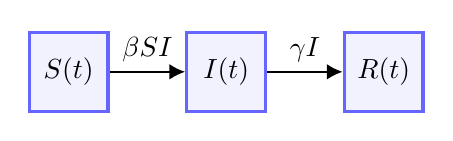
\begin{tikzpicture}[node distance=2cm, auto, thick]
        % Define block styles
        \tikzstyle{block} = [rectangle, draw=blue!60, fill=blue!5, very thick, minimum size=1cm, text centered]
        \tikzstyle{line} = [draw, -{Latex[length=2mm, width=2mm]}]

        % Define nodes
        \node [block] (S) {\( S(t) \)};
        \node [block, right of=S] (I) {\( I(t) \)};
        \node [block, right of=I] (R) { \( R(t) \)};

        % Connect nodes with paths
        \path [line] (S) -- node { \( \beta S I \) } (I);
        \path [line] (I) -- node { \( \gamma I \) } (R);

    \end{tikzpicture}
    \caption{Compartmental flow of the SIR model for infection transmission dynamics.}
\end{figure}

The model operates under the assumption of population conservation, formulated as:
\begin{equation}
    S(t) + I(t) + R(t) = N, \quad \forall t \geq t_0,
\end{equation}
where $N$ denotes the total constant population size. This equation implies that the total number of individuals in the model remains constant over time, encapsulating the assumption that the timescale of the epidemic's evolution is significantly shorter than the average lifespan of individuals in the population. Consequently, demographic processes such as births and natural deaths are not considered, under the premise that their impact on the total population size is negligible within the timeframe of the epidemic's spread.

% \begin{table}[h!]
%     \centering
%     \begin{tabular}{ll}
%     \toprule
%     \textbf{Parameter} & \textbf{Definition} \
%     \midrule
%     $\beta$ & Transmission rate \
%     $\gamma$ & Recovery rate \
%     \bottomrule
%     \end{tabular}
%     \caption{Parameters of the SIR Model}
% \end{table}
    
The SIR model is fundamental in epidemiology for its simplicity and effectiveness in capturing the basic dynamics of disease spread. However, it assumes lifelong immunity post-recovery, which may not apply to all diseases, including COVID-19.

To account for the characteristics of COVID-19, including the existence of a latent period and the possibility of death, the SEIRD model extends the SIR framework by including two additional compartments: Exposed (E) and Dead (D) individuals. The SEIRD model is described by the following differential equations:

\begin{equation}
    \begin{align}
        \frac{dS}{dt} &= -\beta \frac{SI}{N}, \\
        \frac{dE}{dt} &= \beta \frac{SI}{N} - \sigma E, \\
        \frac{dI}{dt} &= \sigma E - \rho I - \alpha I, \\
        \frac{dR}{dt} &= \rho I, \\
        \frac{dD}{dt} &= \alpha I,
    \end{align}
\end{equation}

where $E$ represents the number of exposed individuals who are infected but not yet infectious, and $D$ represents the number of deceased individuals. The parameters $\sigma$, $\rho$, and $\alpha$ represent the rate of exposed individuals becoming infectious, the recovery rate, and the mortality rate, respectively. The total population size is denoted by $N = S + E + I + R + D$. The SEIRD model provides a more comprehensive representation of disease dynamics and is particularly useful for capturing the spread of COVID-19, which exhibits a latent period and the possibility of death. This model more accurately reflects the disease dynamics of COVID-19 by considering the exposed phase, during which individuals are infected but not yet infectious, and the mortality due to the disease. The addition of these compartments allows for a more nuanced understanding of the pandemic's progression and the impact of interventions such as social distancing, vaccination, and treatment strategies.


\begin{figure}[h!]
    \centering
    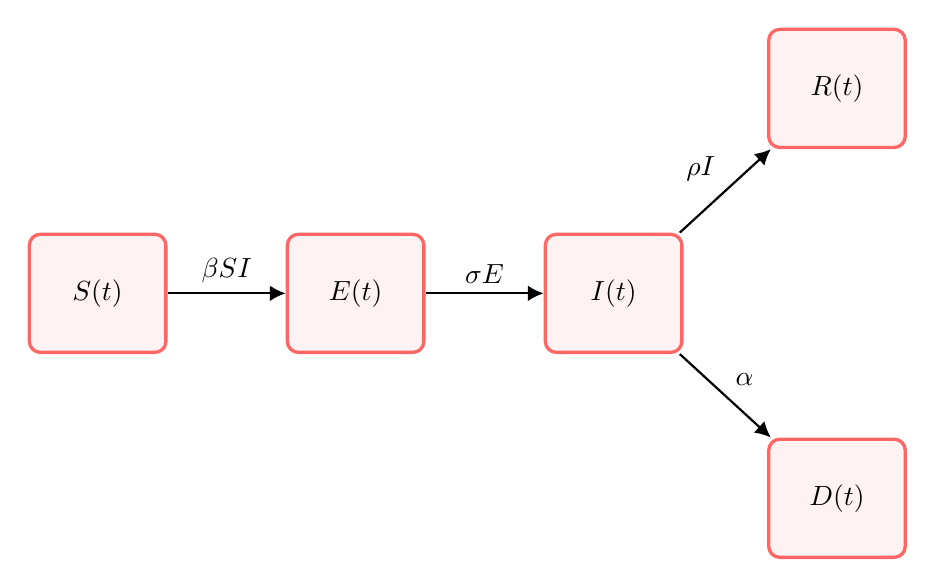
\begin{tikzpicture}[node distance=1.5cm, auto, thick]
        % Define block styles
        \tikzstyle{roundnode} = [circle, draw=green!60, fill=green!5, very thick, minimum size=1cm, text centered]
        \tikzstyle{squarednode} = [rectangle, draw=red!60, fill=red!5, very thick, text width=1.5cm, text centered, rounded corners, minimum height=1.5cm]
        \tikzstyle{line} = [draw, -{Latex[length=2mm, width=2mm]}]
    
        % Define nodes
        \node [squarednode] (S) {\( S(t) \)};
        \node [squarednode, right=of S] (E) {\( E(t) \)};
        \node [squarednode, right=of E] (I) {\( I(t) \)};
        \node [squarednode, above right=of I] (R) { \( R(t) \)};
        \node [squarednode, below right=of I] (D) { \( D(t) \)};
        
        % Connect nodes with paths
        \path [line] (S) -- node { \( \beta S I \) } (E);
        \path [line] (E) -- node { \(  \sigma E \) } (I);
        \path [line] (I) -- node { \( \rho I\) } (R);
        \path [line] (I) -- node { \( \alpha \) } (D);

    \end{tikzpicture}
    \caption{Compartmental flow of the SEIRD model for COVID-19 transmission dynamics.}
\end{figure}

\subsection{Physics-Informed Neural Networks}

Physics-Informed Neural Networks (PINNs) embody a novel approach to embedding a priori system knowledge, such as fundamental physical principles or domain expertise, directly into the learning mechanism of deep neural networks. This incorporation is typically achieved through the utilization of ordinary or partial differential equations (ODEs/PDEs) within the loss function formulation. During training, PINNs aim not only to adjust network weights and biases but also to refine parameters within the encapsulated physical laws. The composite loss function encompasses two primary components: the data fidelity loss ($L_{\text{data}}$) and the physics-based residual loss ($L_{\text{residual}}$), the latter serving as a regularization mechanism that enforces adherence to established differential equations.

Consider a system governed by a set of first-order ODEs expressed as:
\begin{equation}
\frac{\partial U}{\partial t}(t) + F(U(t); \lambda) = 0, \quad t \in [t_0, T],
\end{equation}
where $U(t) = [u_1(t), \ldots, u_n(t)]^T$ and $F(U) = [f_1(U), \ldots, f_n(U)]^T$ with $u_i \in \mathbb{R}$ and $f_i: \mathbb{R}^n \rightarrow \mathbb{R}$ for $i = 1, \ldots, n$. The interval $[t_0, T]$ denotes the time domain from initial to final time, with $\lambda \in \mathbb{R}^k$ representing unknown parameters of the system. The observed data $U_s$ at times $t_1, \ldots, t_m$ are used to determine $\lambda$, leading to the data loss:
\begin{equation}
L_{\text{data}} = \sum_{s=1}^{m} \|U(t_s) - U_s\|^2.
\end{equation}

Traditionally, the optimal parameter vector $\lambda$ is identified by minimizing $L_{\text{data}}$, thereby deriving a solution $U(t)$ that closely aligns with the observed data in terms of least squares deviations. PINNs leverage a general neural network framework, denoted as $NN_{\omega,b}(t): \mathbb{R} \rightarrow \mathbb{R}^n$, which approximates the solution $U(t): \mathbb{R} \rightarrow \mathbb{R}^n$ of the ODE system. The network's weights $\omega$ and biases $b$ are optimized to minimize the mean squared error (MSE) between the network's predictions and the observed data:

\begin{equation}[h]
    MSE_{\omega,b}^U = \frac{1}{m} \sum_{s=1}^{m} \|NN_{\omega,b}(t_s) - U_s\|^2.
\end{equation}

The residual loss, derived from the system of ODEs, is formulated as:
\begin{equation}
F(NN_{\omega,b}, t; \lambda) = \frac{\partial NN_{\omega,b}}{\partial t}(t) + F(NN_{\omega,b}(t); \lambda),
\end{equation}
enabling the extension of $NN_{\omega,b}$ into a PINN by incorporating the residual term into the loss function. Through automatic differentiation, the neural network computes derivatives of its output with respect to its input, thus ensuring compliance with the ODE dynamics by enforcing $F(NN_{\omega,b}, t; \lambda) = 0$ for all $t \in [t_0, T]$. Consequently, PINNs facilitate the simultaneous identification of optimal neural network parameters ($\omega$ and $b$) and ODE parameters ($\lambda$), through the minimization of the combined loss:
\begin{equation}
\text{arg min}_{\omega, b, \lambda} \left( MSE_{\omega,b}^U + MSE_{\omega,b,\lambda}^F \right),
\end{equation}
where $MSE_{\omega,b,\lambda}^F$ represents the mean squared residual error, integrating the system's dynamics into the optimization process.

\begin{figure}
    \centering
    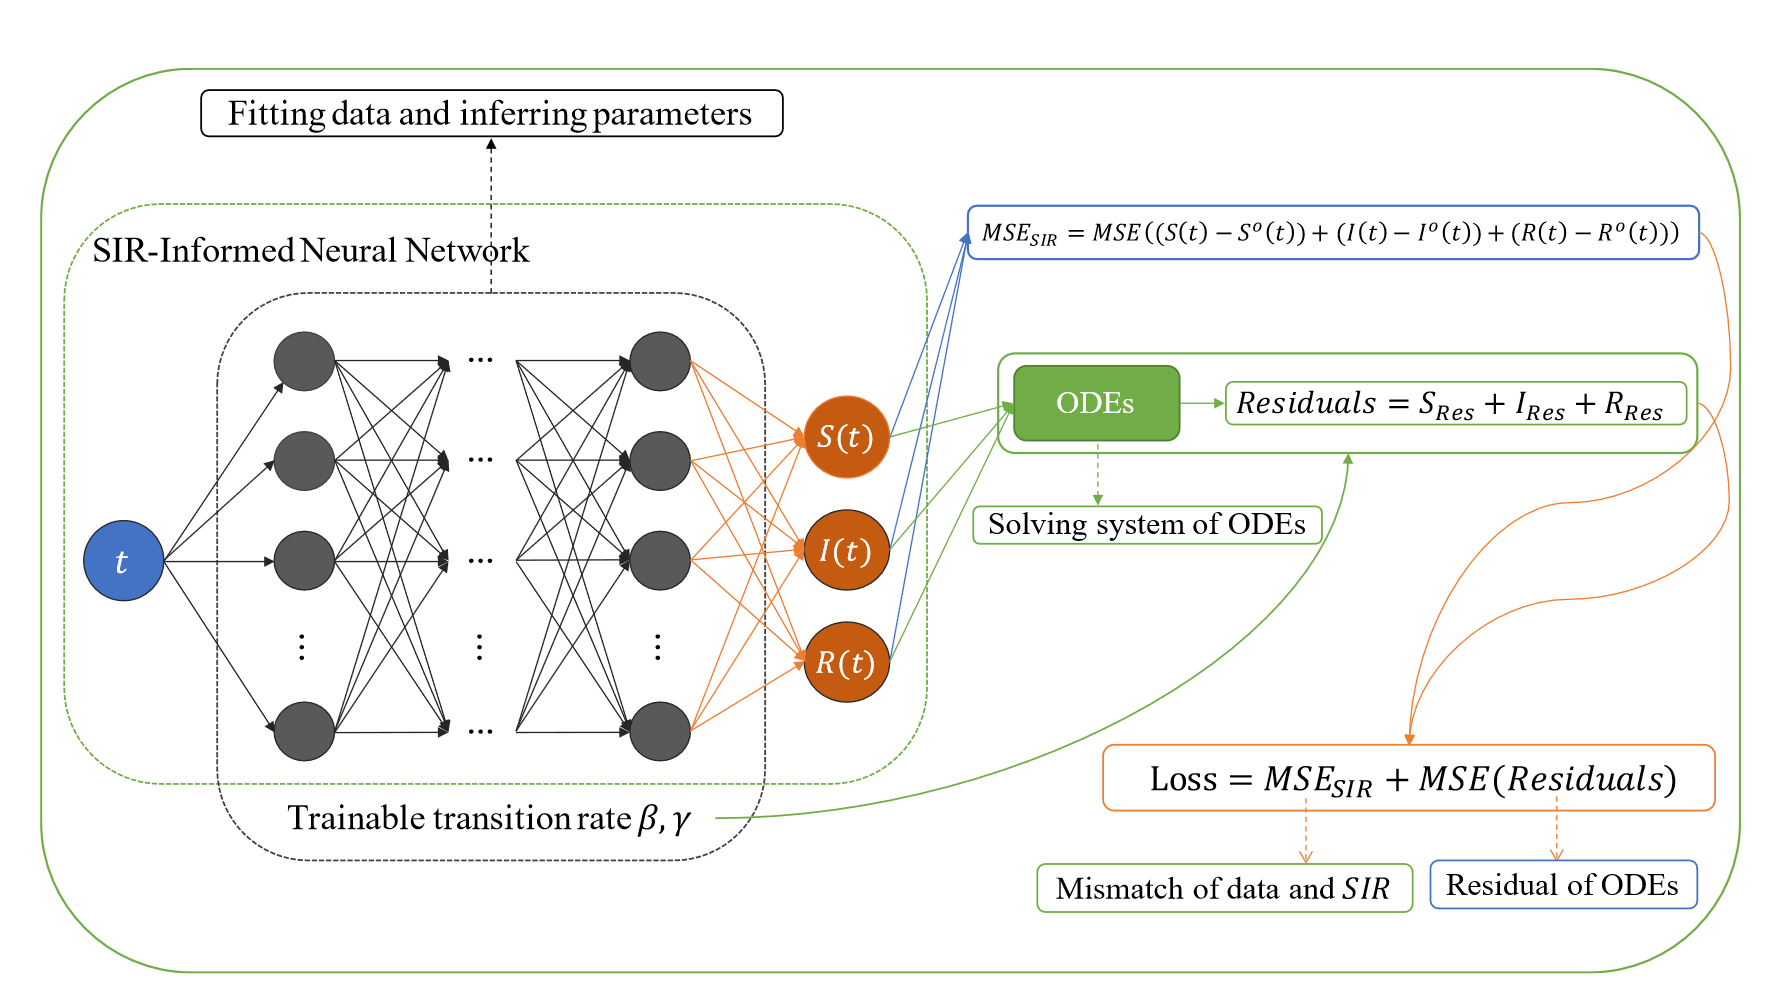
\includegraphics[width=0.8\textwidth]{images/image.png}
    \caption{Caption}
    \label{fig:enter-label}
\end{figure}

\begin{algorithm}[ht]
    \label{alg:PINN}
    \caption{Training of Physics-Informed Neural Network (PINN) for Epidemic Modeling}
    \begin{algorithmic}[1]
        \Require Training data tensors $\bm{S}_{\text{data}}$, $\bm{I}_{\text{data}}$, $\bm{R}_{\text{data}}$, time tensor $\bm{t}_{\text{data}}$, population size $N$.
        \State Initialize a PINN model $NN$ with Xavier initialization.

        \State Configure the Adam optimizer with a specified learning rate and weight decay.
        
        \For{$epoch = 1$ to $num\_epochs$}
        
            \State Forward pass: $\bm{S}_{\text{pred}}$, $\bm{I}_{\text{pred}}$, $\bm{R}_{\text{pred}} \gets NN(\bm{t}_{\text{data}})$.
            
            \State Calculate gradients via automatic differentiation.
            
            \State Compute mean squared error $MSE_{SIR}$ between predictions and data.
            
            \[ MSE_{SIR} = \frac{1}{s}\sum_{i=1}^{s} \left((S_i - S_{i, \text{data}})^2 + (I_i - I_{i, \text{data}})^2 + (R_i - R_{i, \text{data}})^2\right). \]
            
            \State Calculate residuals' mean squared error $MSE_{residuals}$.
            
            \[ MSE_{residuals} = \frac{1}{q}\sum_{i=1}^{q} \left(\left|\frac{dS_i}{dt} + \frac{\beta S_i I_i}{N}\right|^2 + \left|\frac{dI_i}{dt} - \frac{\beta S_i I_i}{N} + \gamma I_i\right|^2 + \left|\frac{dR_i}{dt} - \gamma I_i\right|^2\right). \]


            \[Loss = MSE_{SIR} + MSE_{residuals}\].
            
            \State Update model weights by backpropagation and optimization.
            \State Apply learning rate scheduler and early stopping if conditions are met.
            
        \EndFor
    \end{algorithmic}
\end{algorithm}


\section{Results and Discussion}




\section{Conclusion}


\begin{algorithm}
\caption{Parameter Estimation for SEIRD Model via Differential Equation Learning}
\begin{algorithmic}[1]

\Require Time series data, population data, initial infected and death counts.

\State Normalize and partition data for model inputs.

\State Initialize model states $u(t_0) = [S_0, E_0, I_0, R_0, D_0]$.

\State Discretize time domain into $t_1, t_2, \ldots, t_n$.

\State Construct neural networks $NN_{\beta}(t;\theta_{\beta})$, $NN_{\gamma}(t;\theta_{\gamma})$, $NN_{\delta}(t;\theta_{\delta})$, $NN_{\alpha}(t;\theta_{\alpha})$ with parameters $\theta_{\beta}$, $\theta_{\gamma}$, $\theta_{\delta}$, $\theta_{\alpha}$.

\State Define the SEIRD differential equations with learned parameters:
\Function{SEIRD}{$\dot{u}, u, \theta, t$}
    \State $\beta(t), \gamma(t), \delta(t), \alpha(t) \gets |NN_{\beta}(t;\theta_{\beta})|, |NN_{\gamma}(t;\theta_{\gamma})|, |NN_{\delta}(t;\theta_{\delta})|, |NN_{\alpha}(t;\theta_{\alpha})|$
    \State $\dot{S}, \dot{E}, \dot{I}, \dot{R}, \dot{D} \gets \text{transitions based on SEIRD dynamics and } \beta(t), \gamma(t), \delta(t), \alpha(t)$
\EndFunction

\State Formulate the initial value problem (IVP) using $u(t_0)$ and SEIRD dynamics.

\State Define loss function $\mathcal{L}(\theta)$ combining prediction errors and parameter trajectory regularizations.

\State Minimize $\mathcal{L}(\theta)$ using gradient-based optimization with callbacks to monitor convergence.

\State Evaluate model fit with metrics such as MSE, MAE, MAPE, RMSE.

\end{algorithmic}
\end{algorithm}



\begin{tabular}{ll}
\toprule
\textbf{Parameter} & \textbf{Definition} \\
\midrule
$\beta$ & Transmission rate \\
$\delta$ & Rate at which exposed individuals become infectious \\
$\gamma$ & Recovery rate \\
$\alpha$ & Mortality rate \\
\bottomrule
\end{tabular}

\begin{figure*}[ht]
    \centering
    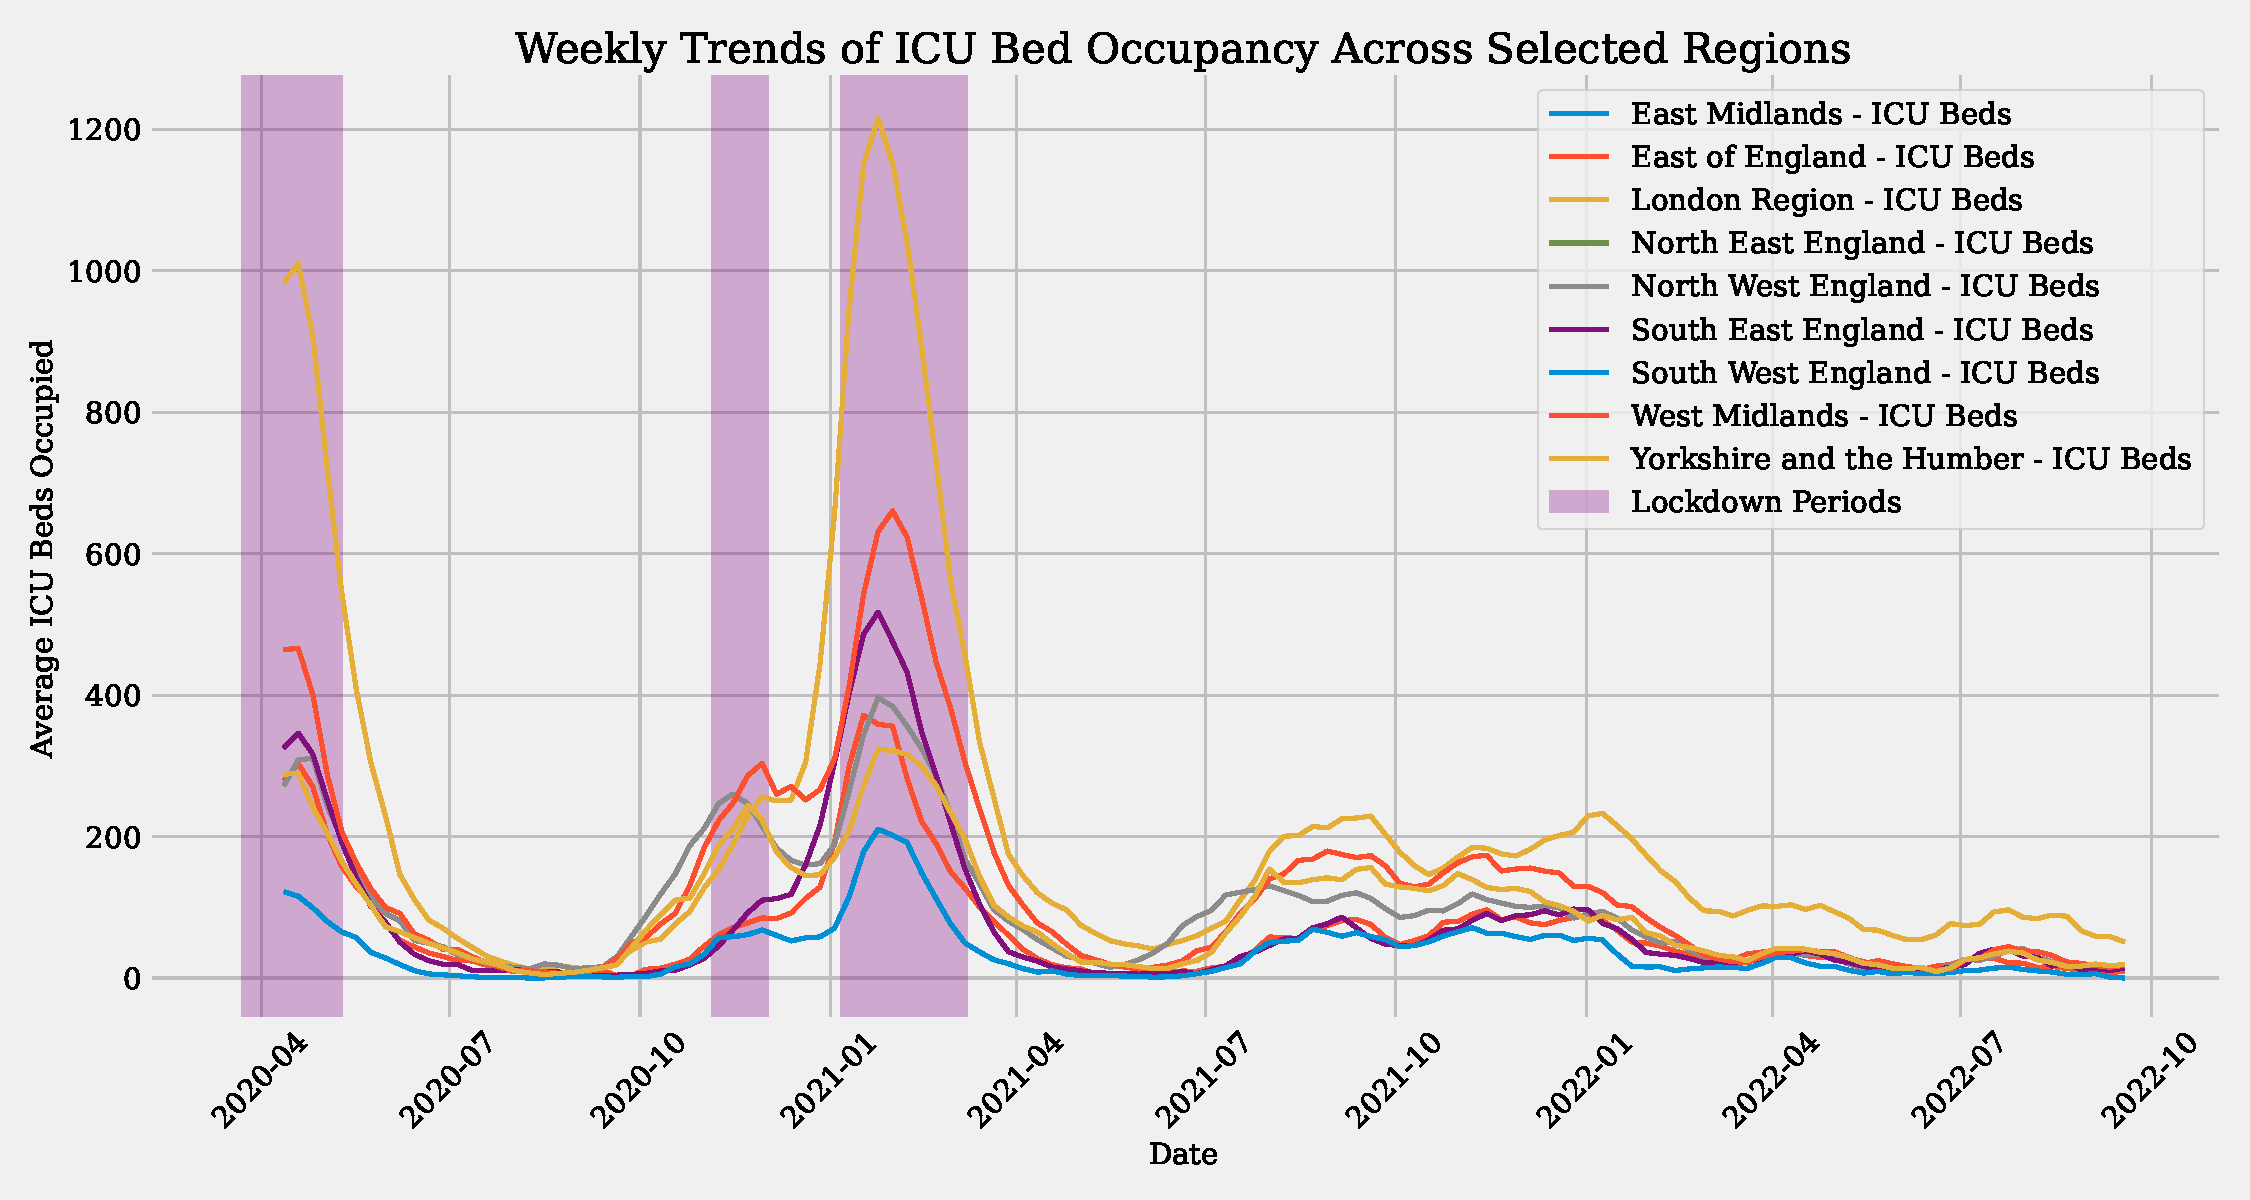
\includegraphics[width=0.8\textwidth]{"images/weekly_icu_beds_occupancy.pdf"}
    \caption{weekly ICU bed occupancy across NHS regions.}
    \label{fig:ICU_beds_occupancy}
\end{figure*}


\begin{figure*}[ht]
    \centering
    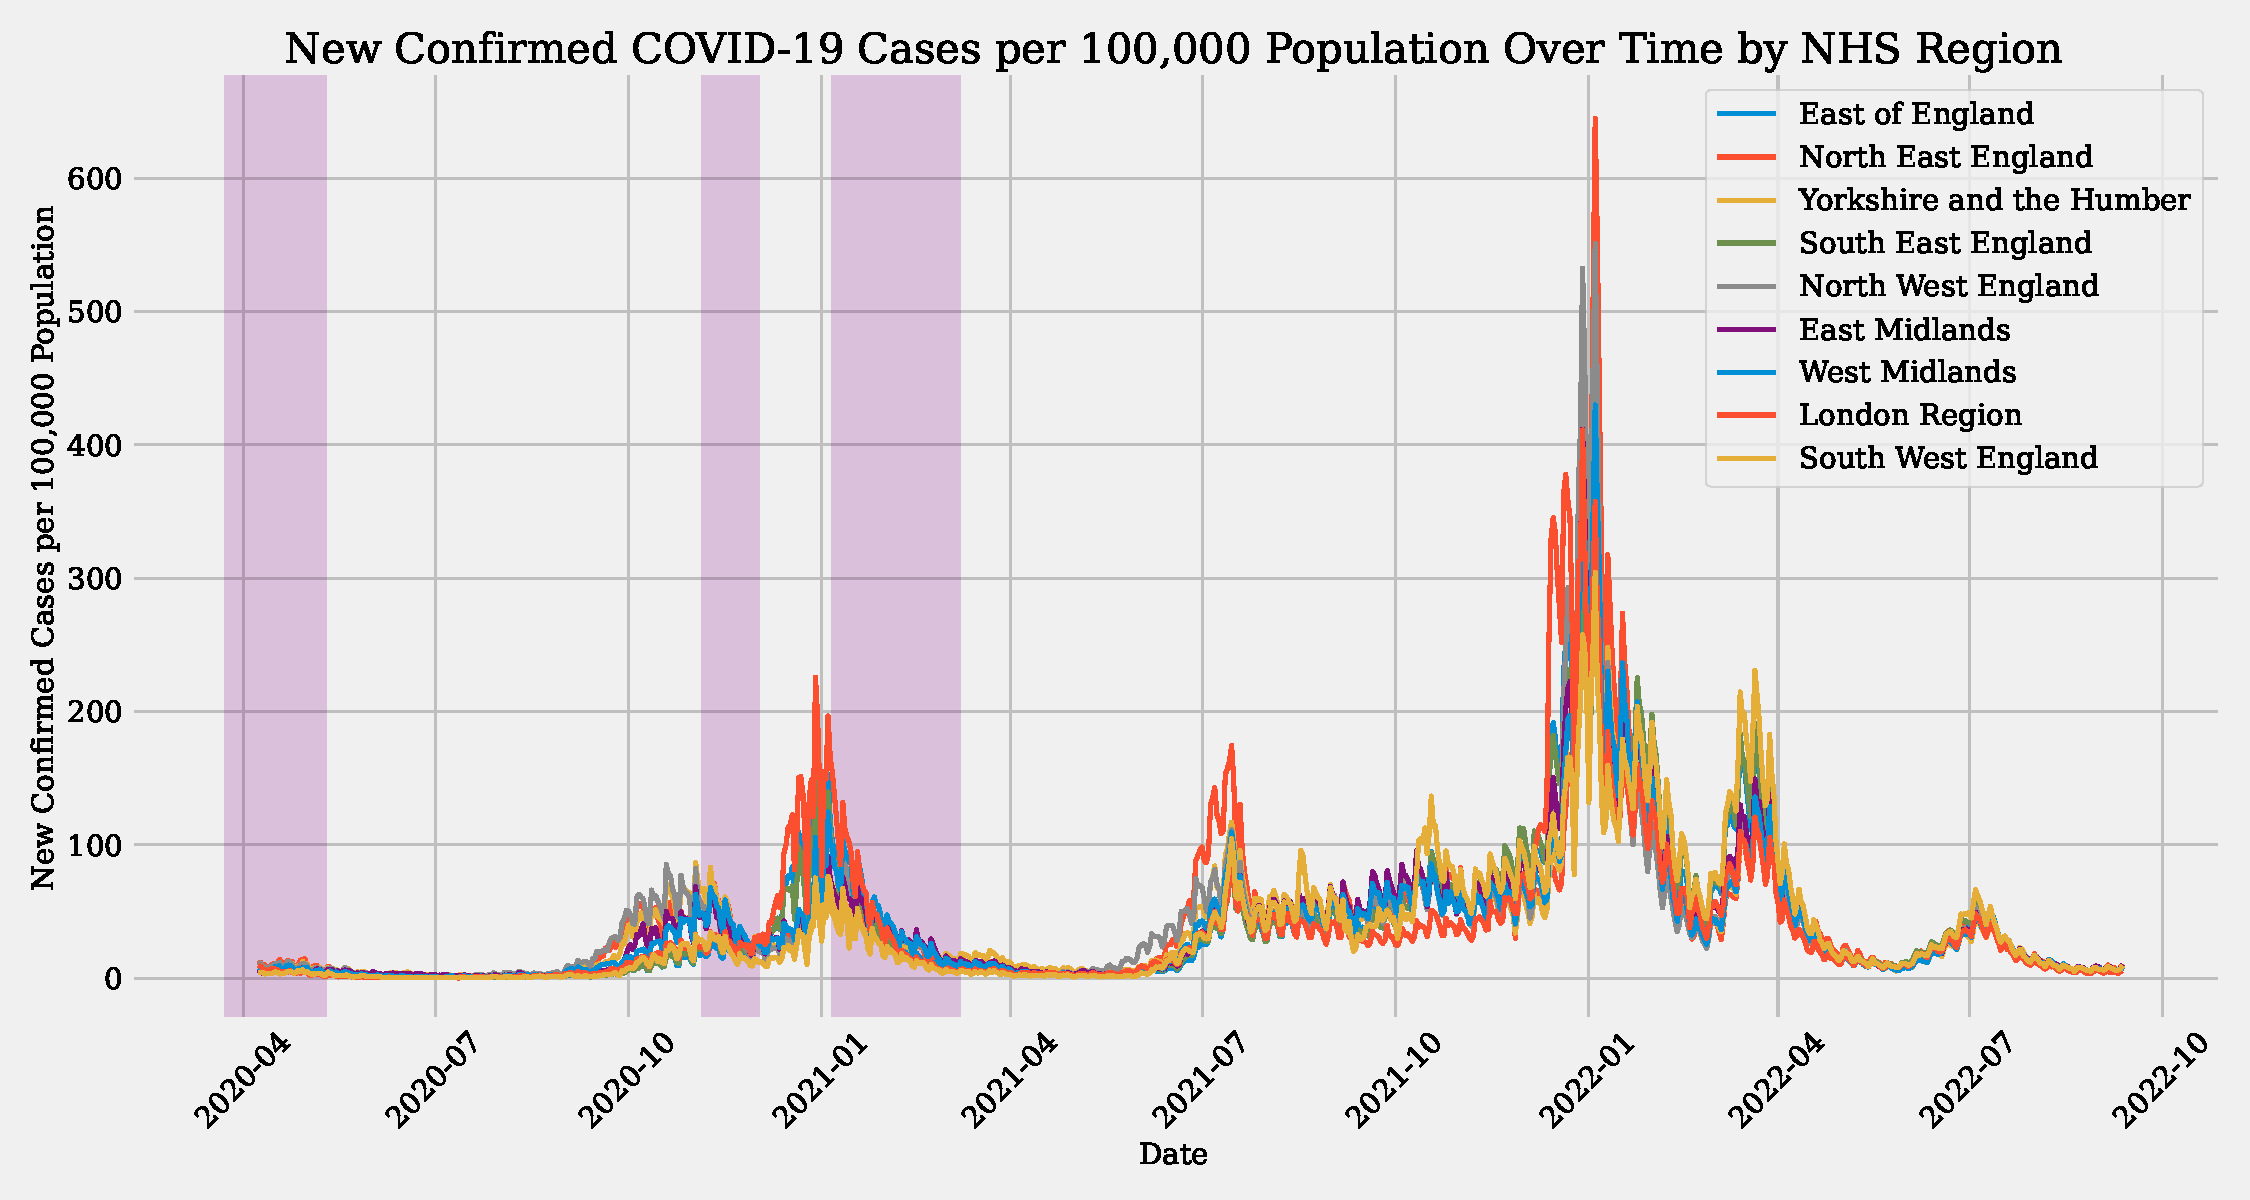
\includegraphics[width=0.8\textwidth]{"images/new_confirmed_per_100k.pdf"}
    \caption{new confirmed COVID-19 cases per 100k people overtime by NHS regions.}
    \label{fig:new_confirmed_per_100k}
\end{figure*}

\begin{figure*}[ht]
    \centering
    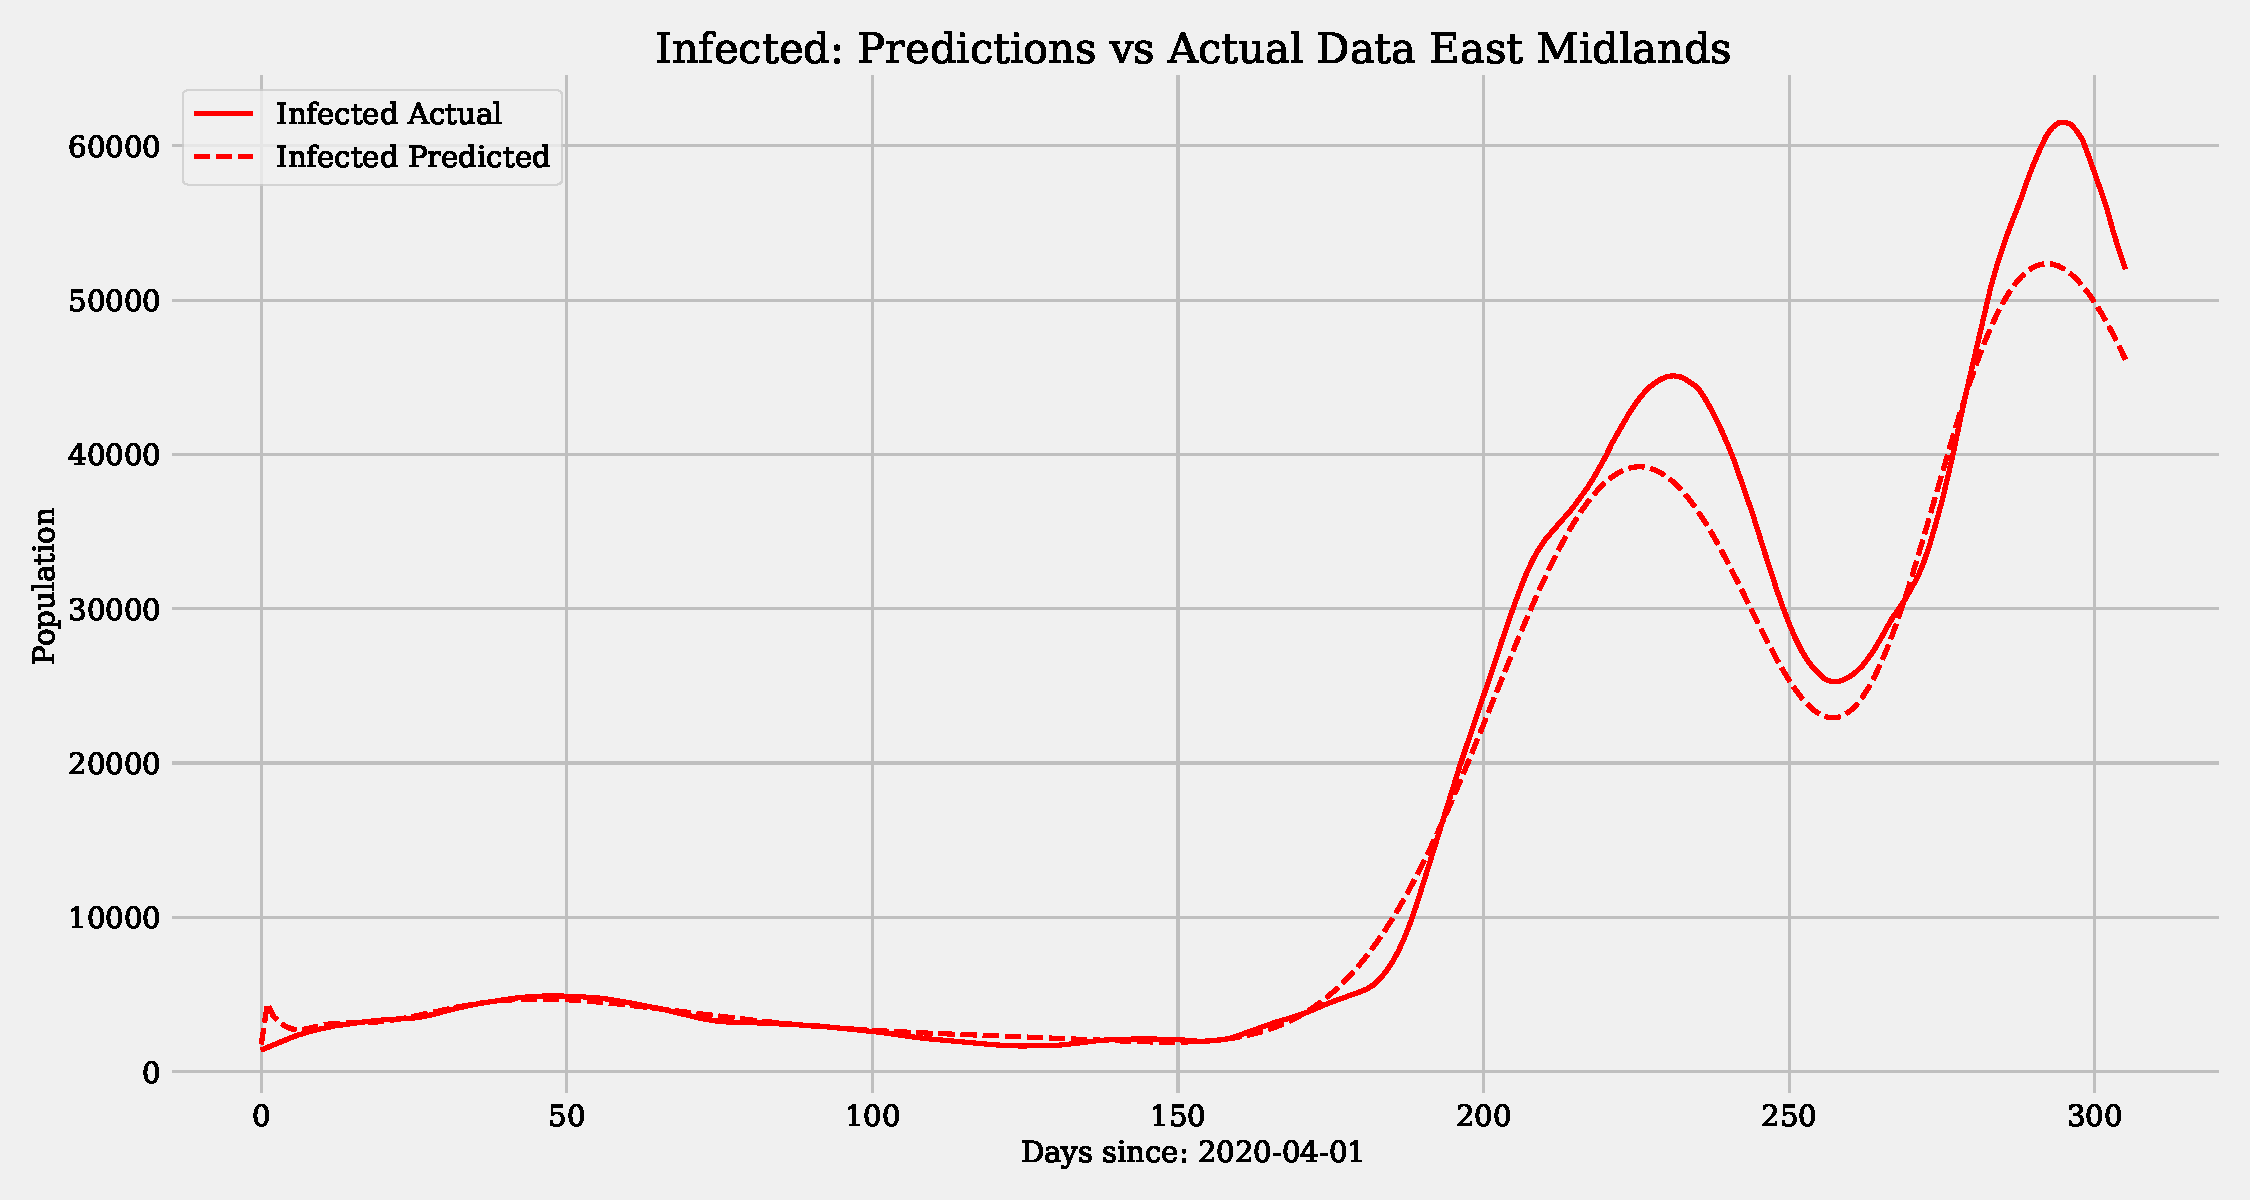
\includegraphics[width=0.8\textwidth]{images/pinn/I_predictions_East Midlands.pdf}
    \caption{Predicted number of infectious individuals in the East Midlands region.}
    \label{fig:I_predictions_East_Midlands}
\end{figure*}

\begin{figure*}[ht]
    \centering
    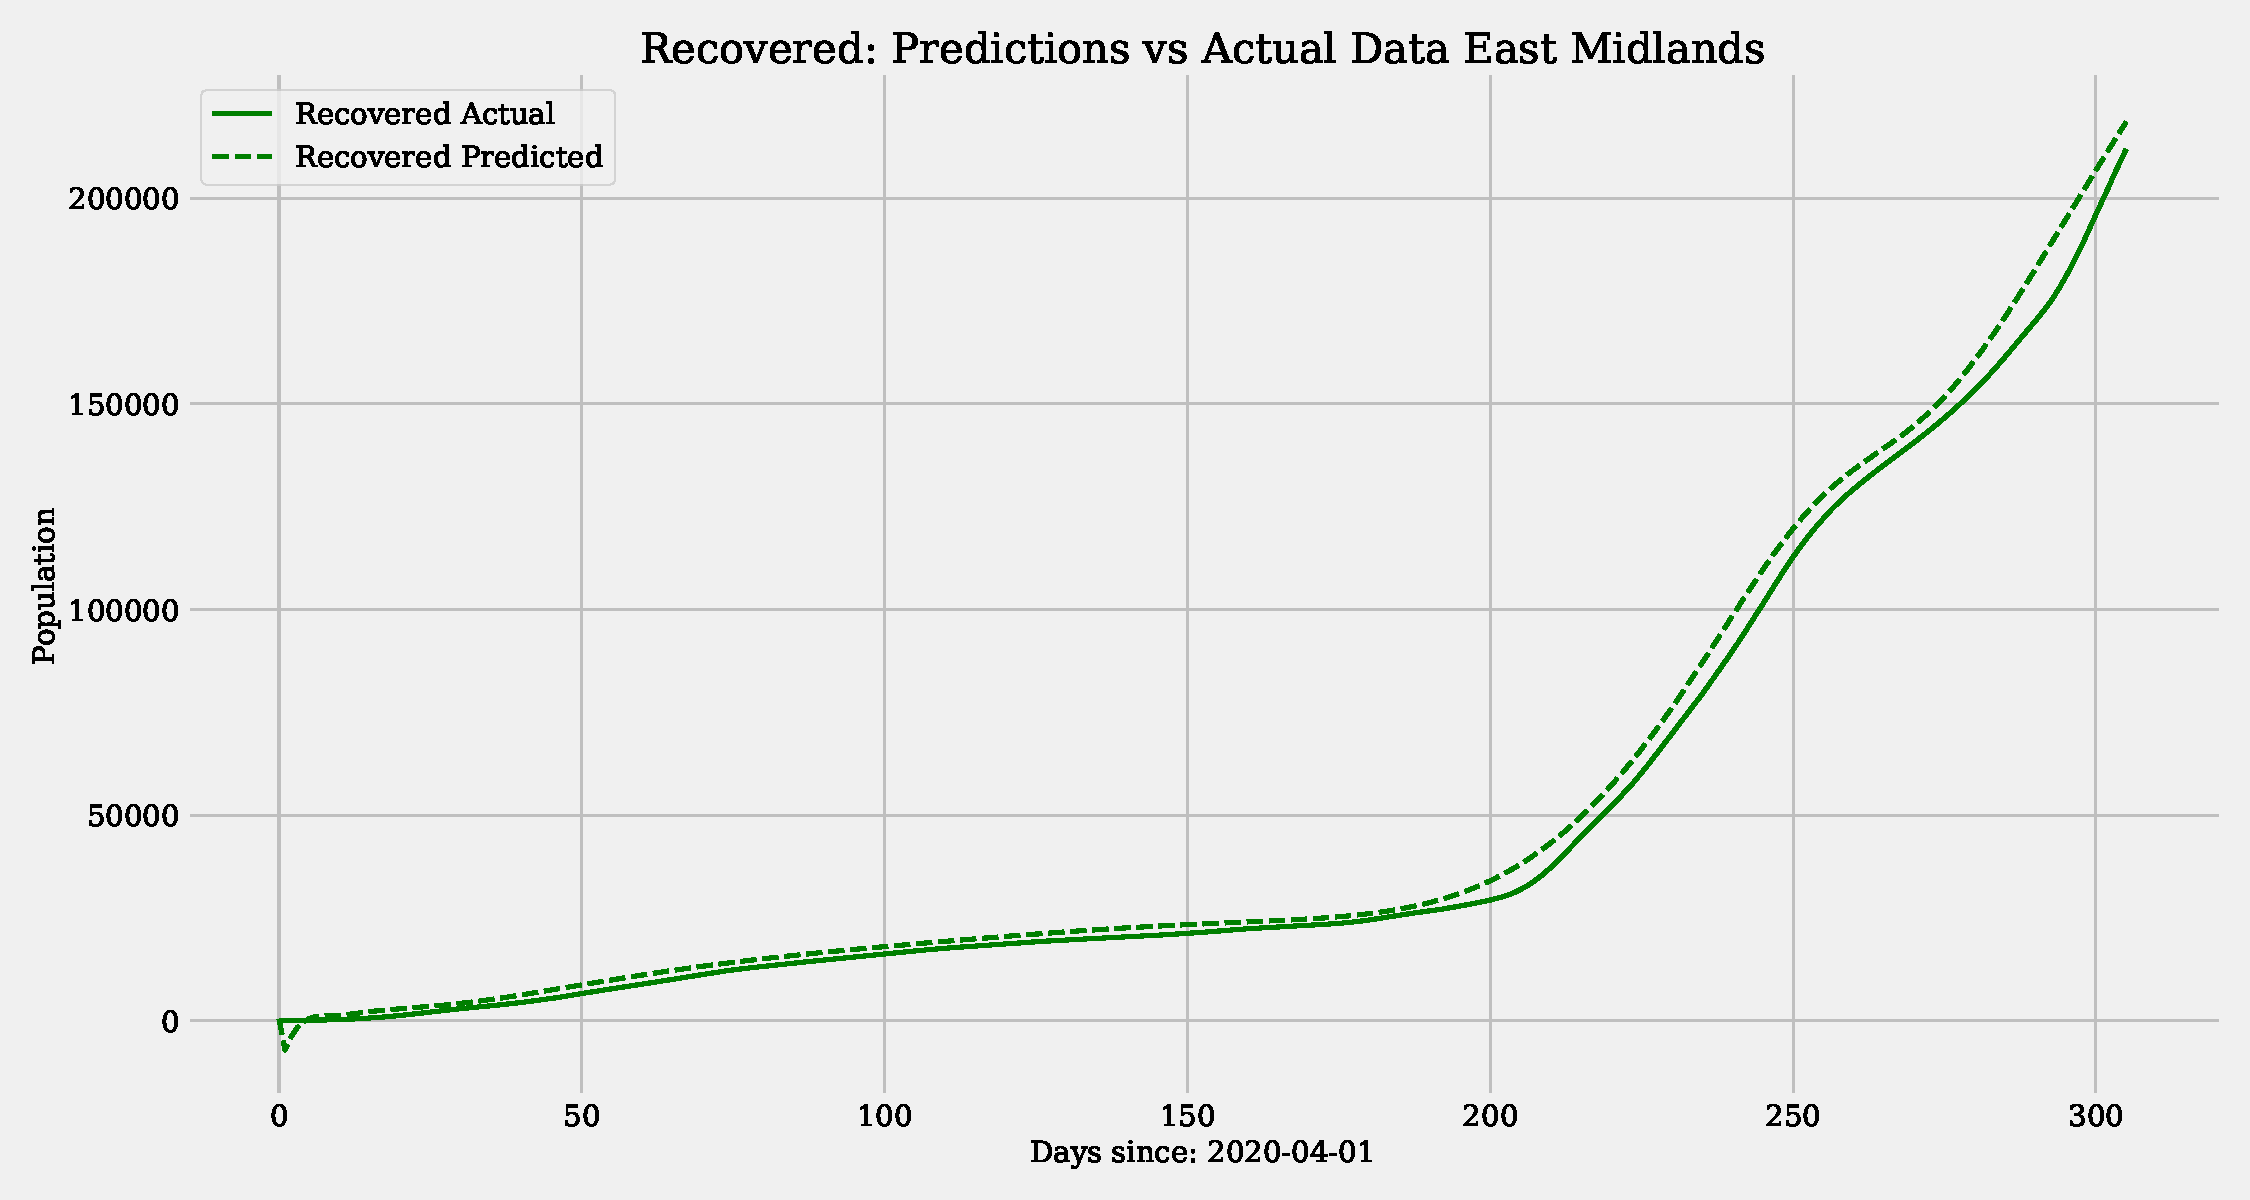
\includegraphics[width=0.8\textwidth]{images/pinn/R_predictions_East Midlands.pdf}
    \caption{Predicted number of recovered individuals in the East Midlands region.}
    \label{fig:R_predictions_East_Midlands}
\end{figure*}

\begin{figure*}[ht]
    \centering
    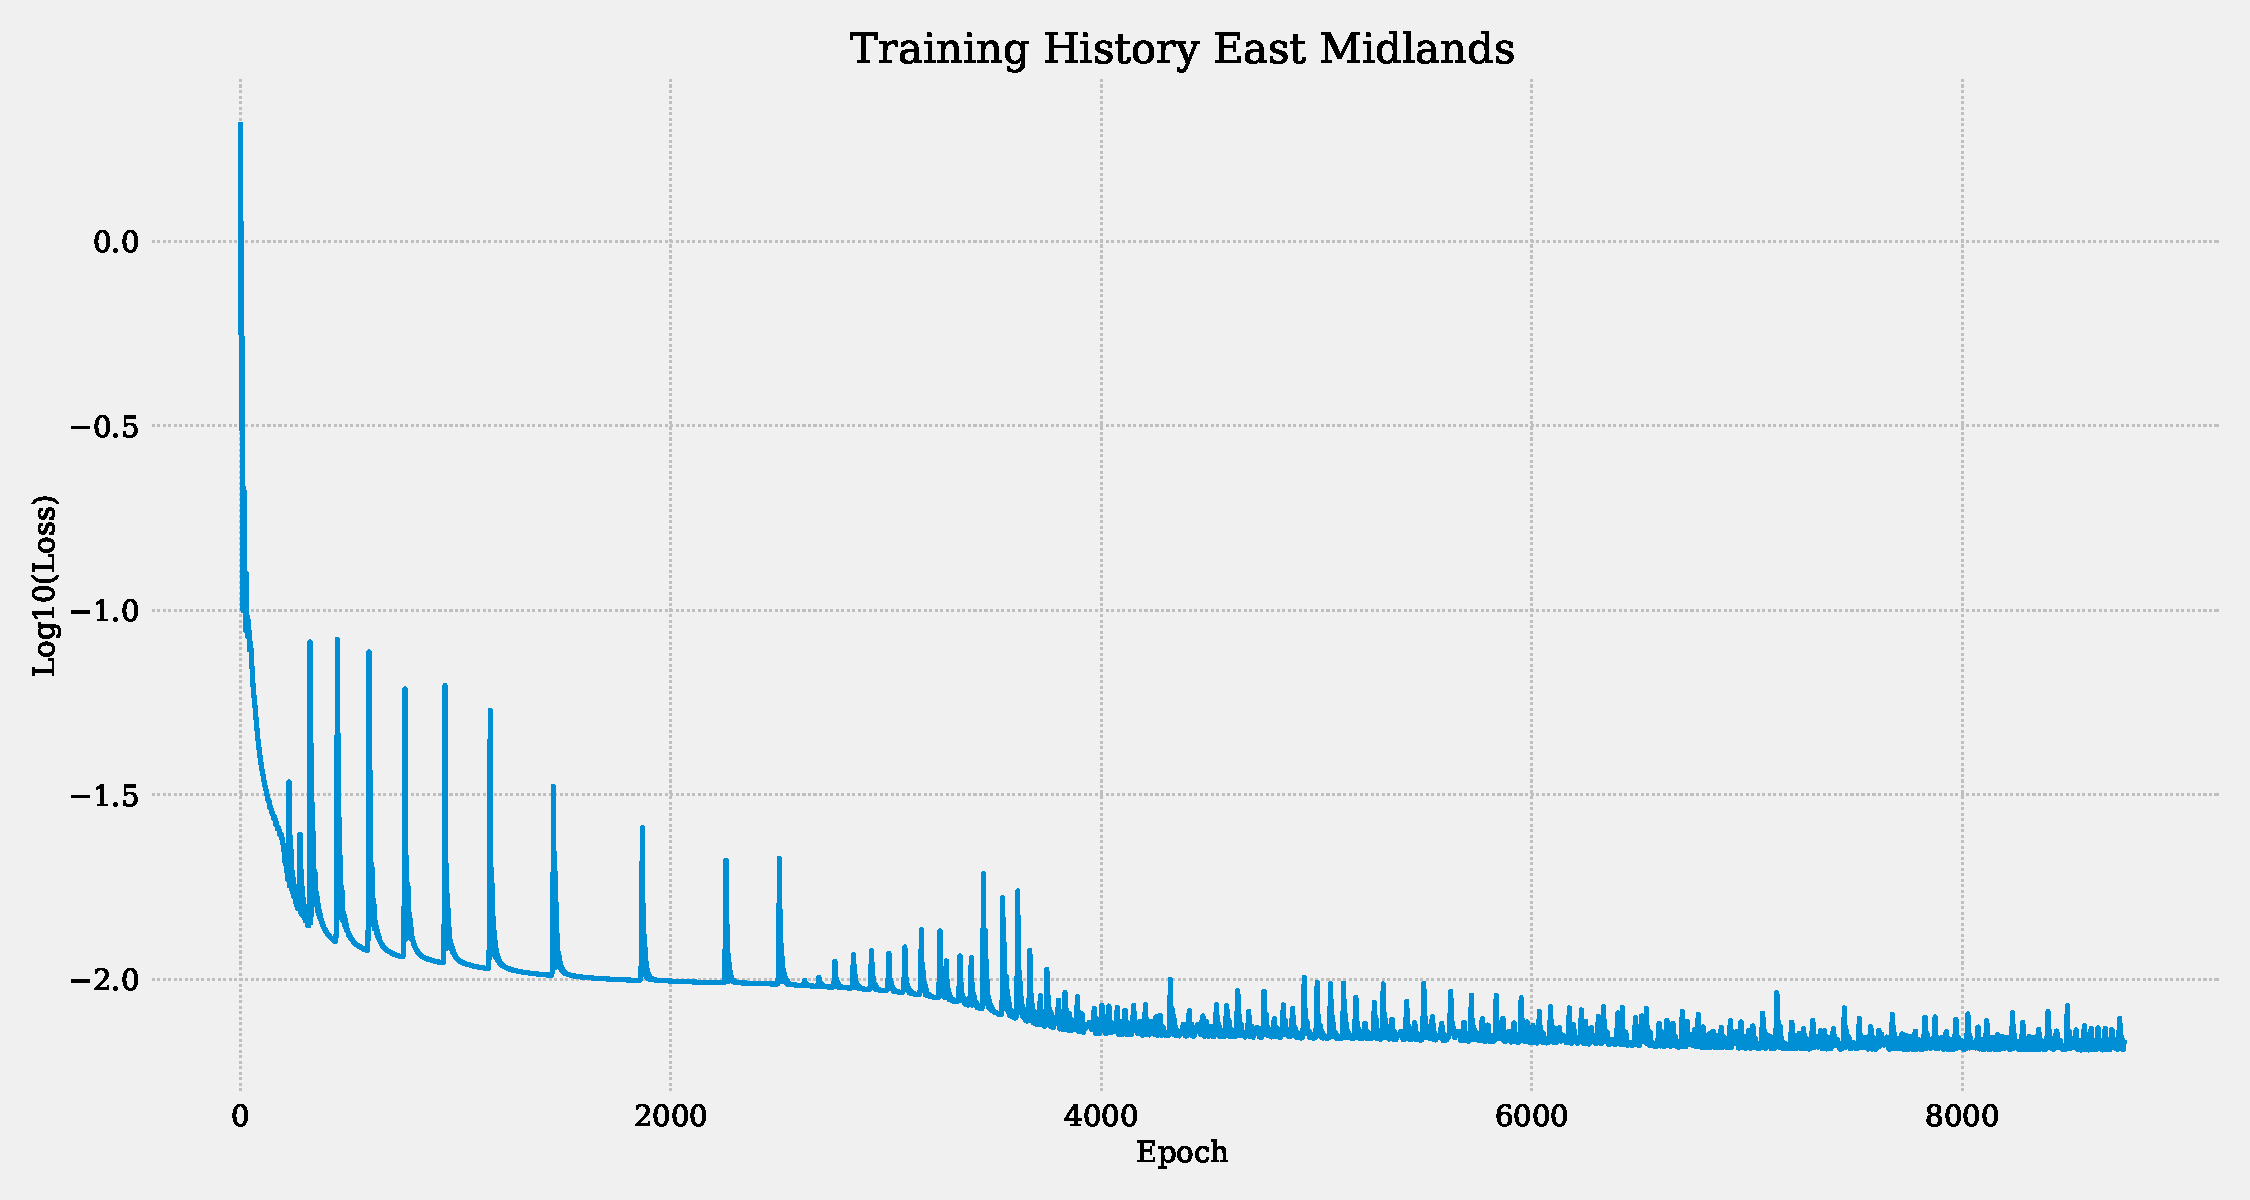
\includegraphics[width=0.8\textwidth]{images/pinn/Training_History_East Midlands.pdf}
    \caption{Training history of the PINN model for the East Midlands region.}
    \label{fig:Training_History_East_Midlands}
\end{figure*}

\begin{figure*}[ht]
    \centering
    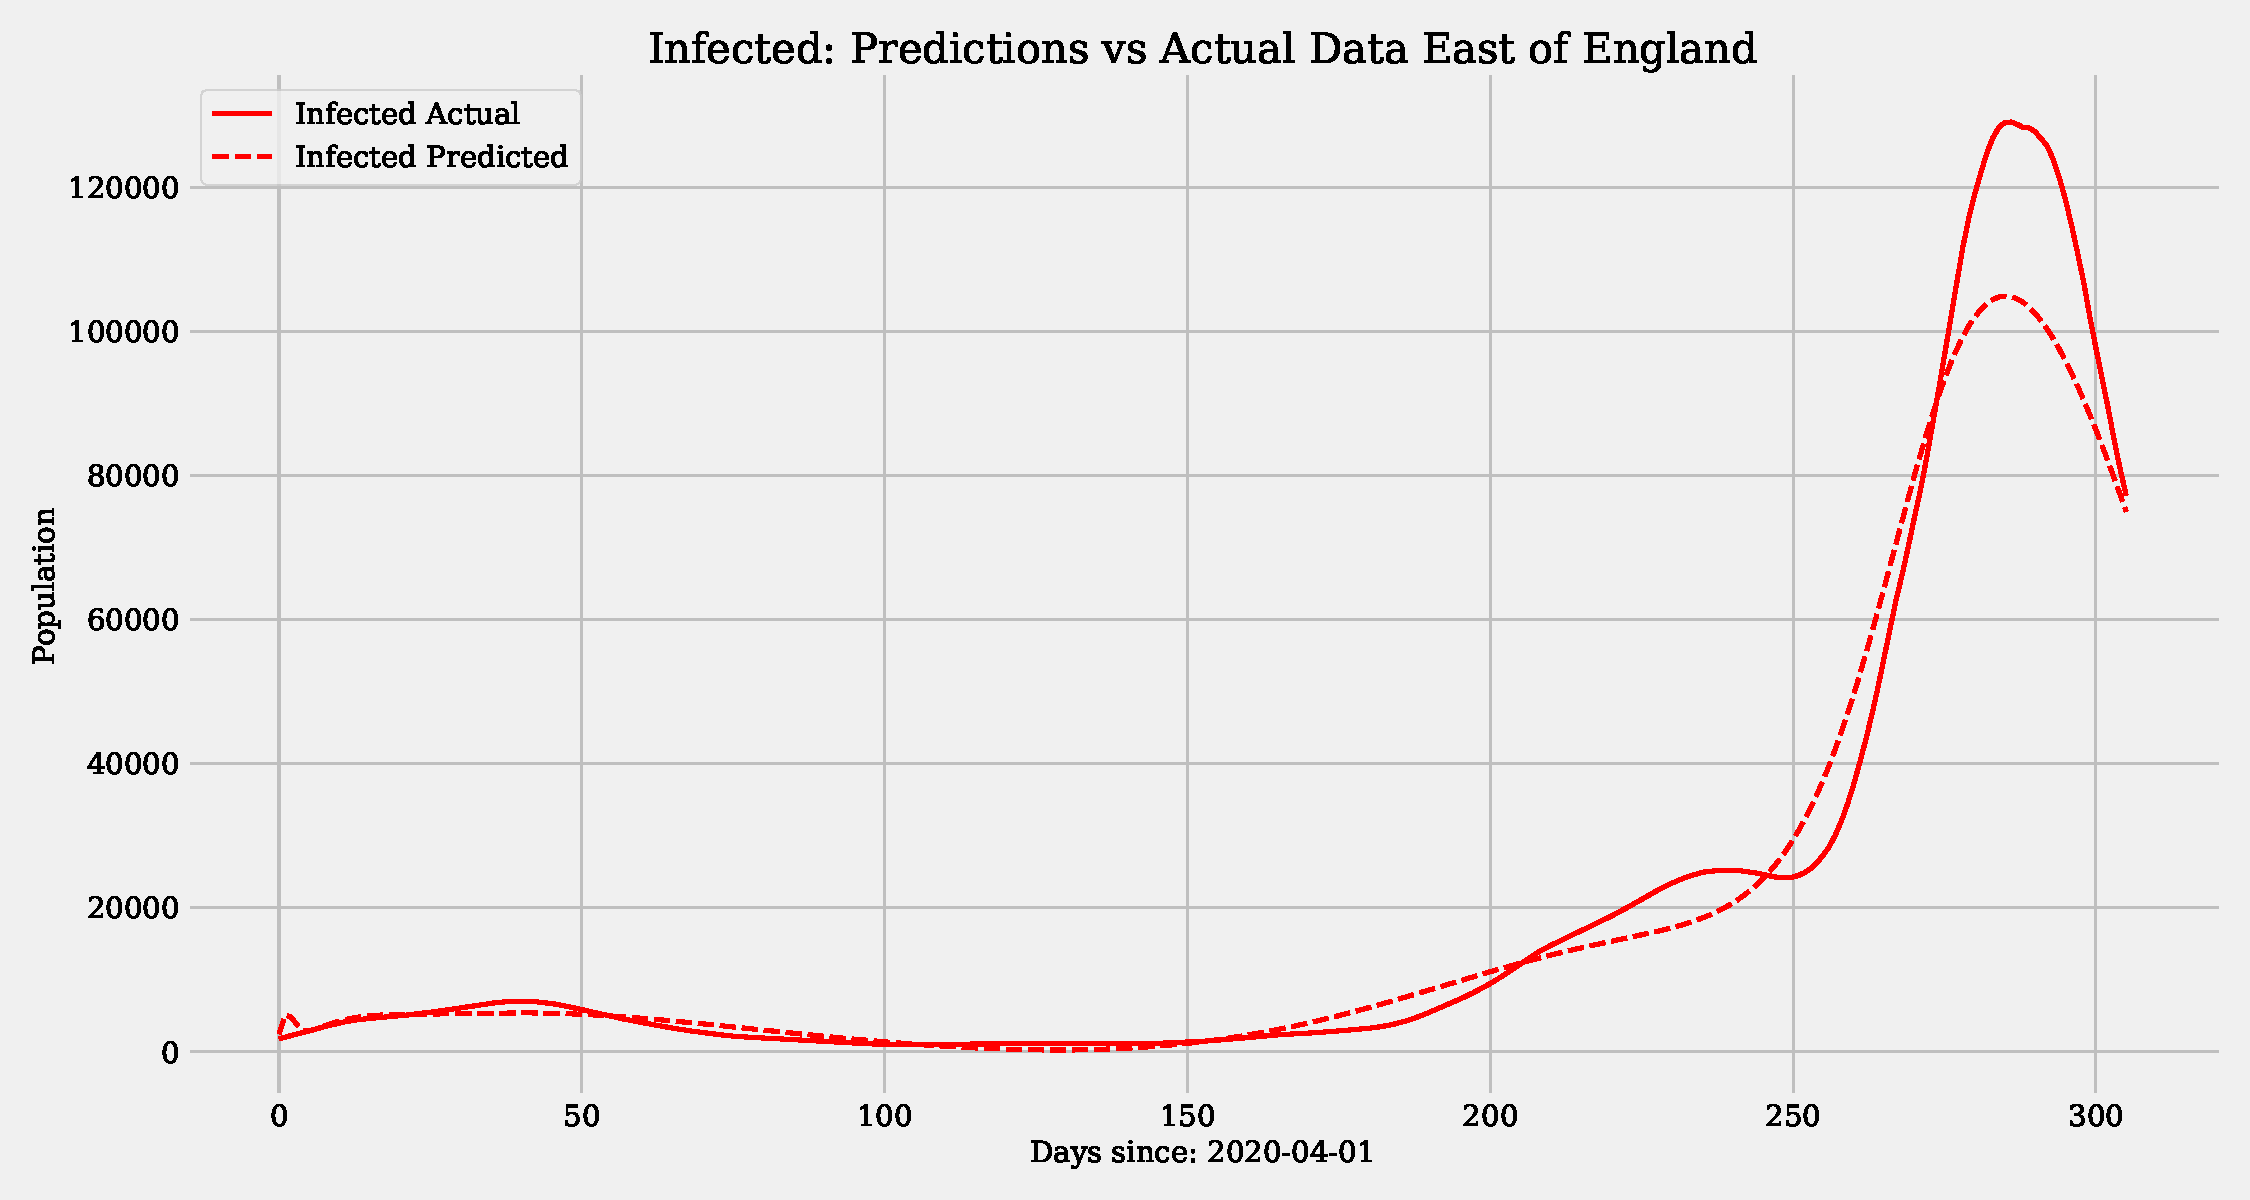
\includegraphics[width=0.8\textwidth]{images/pinn/I_predictions_East of England.pdf}
    \caption{Predicted number of infectious individuals in the East of England region.}
    \label{fig:I_predictions_East_of_England}
\end{figure*}

\begin{figure*}[ht]
    \centering
    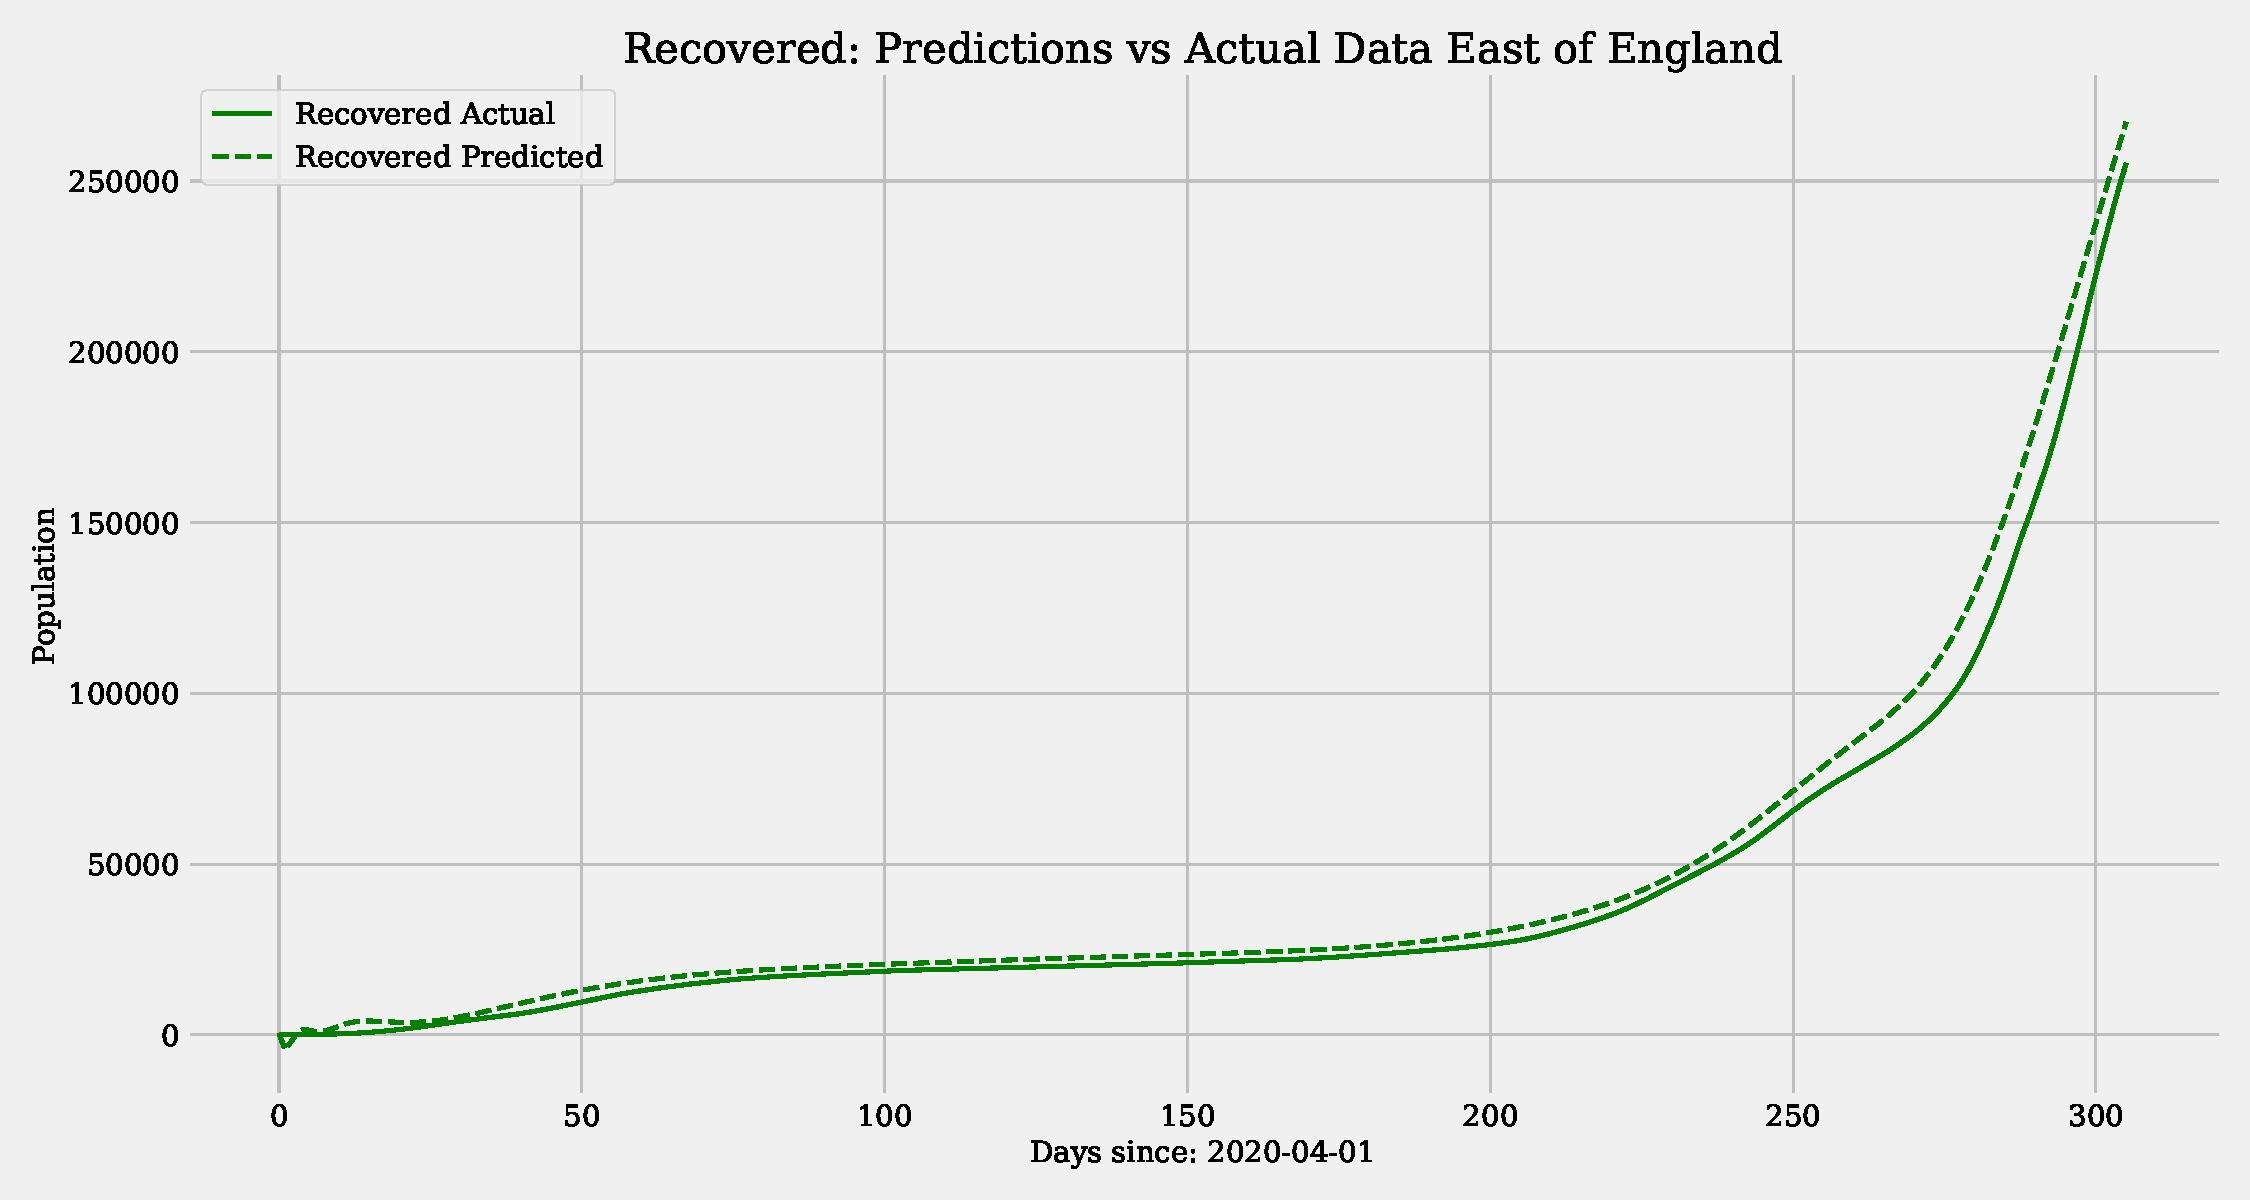
\includegraphics[width=0.8\textwidth]{images/pinn/R_predictions_East of England.pdf}
    \caption{Predicted number of recovered individuals in the East of England region.}
    \label{fig:R_predictions_East_of_England}
\end{figure*}

\begin{figure*}[ht]
    \centering
    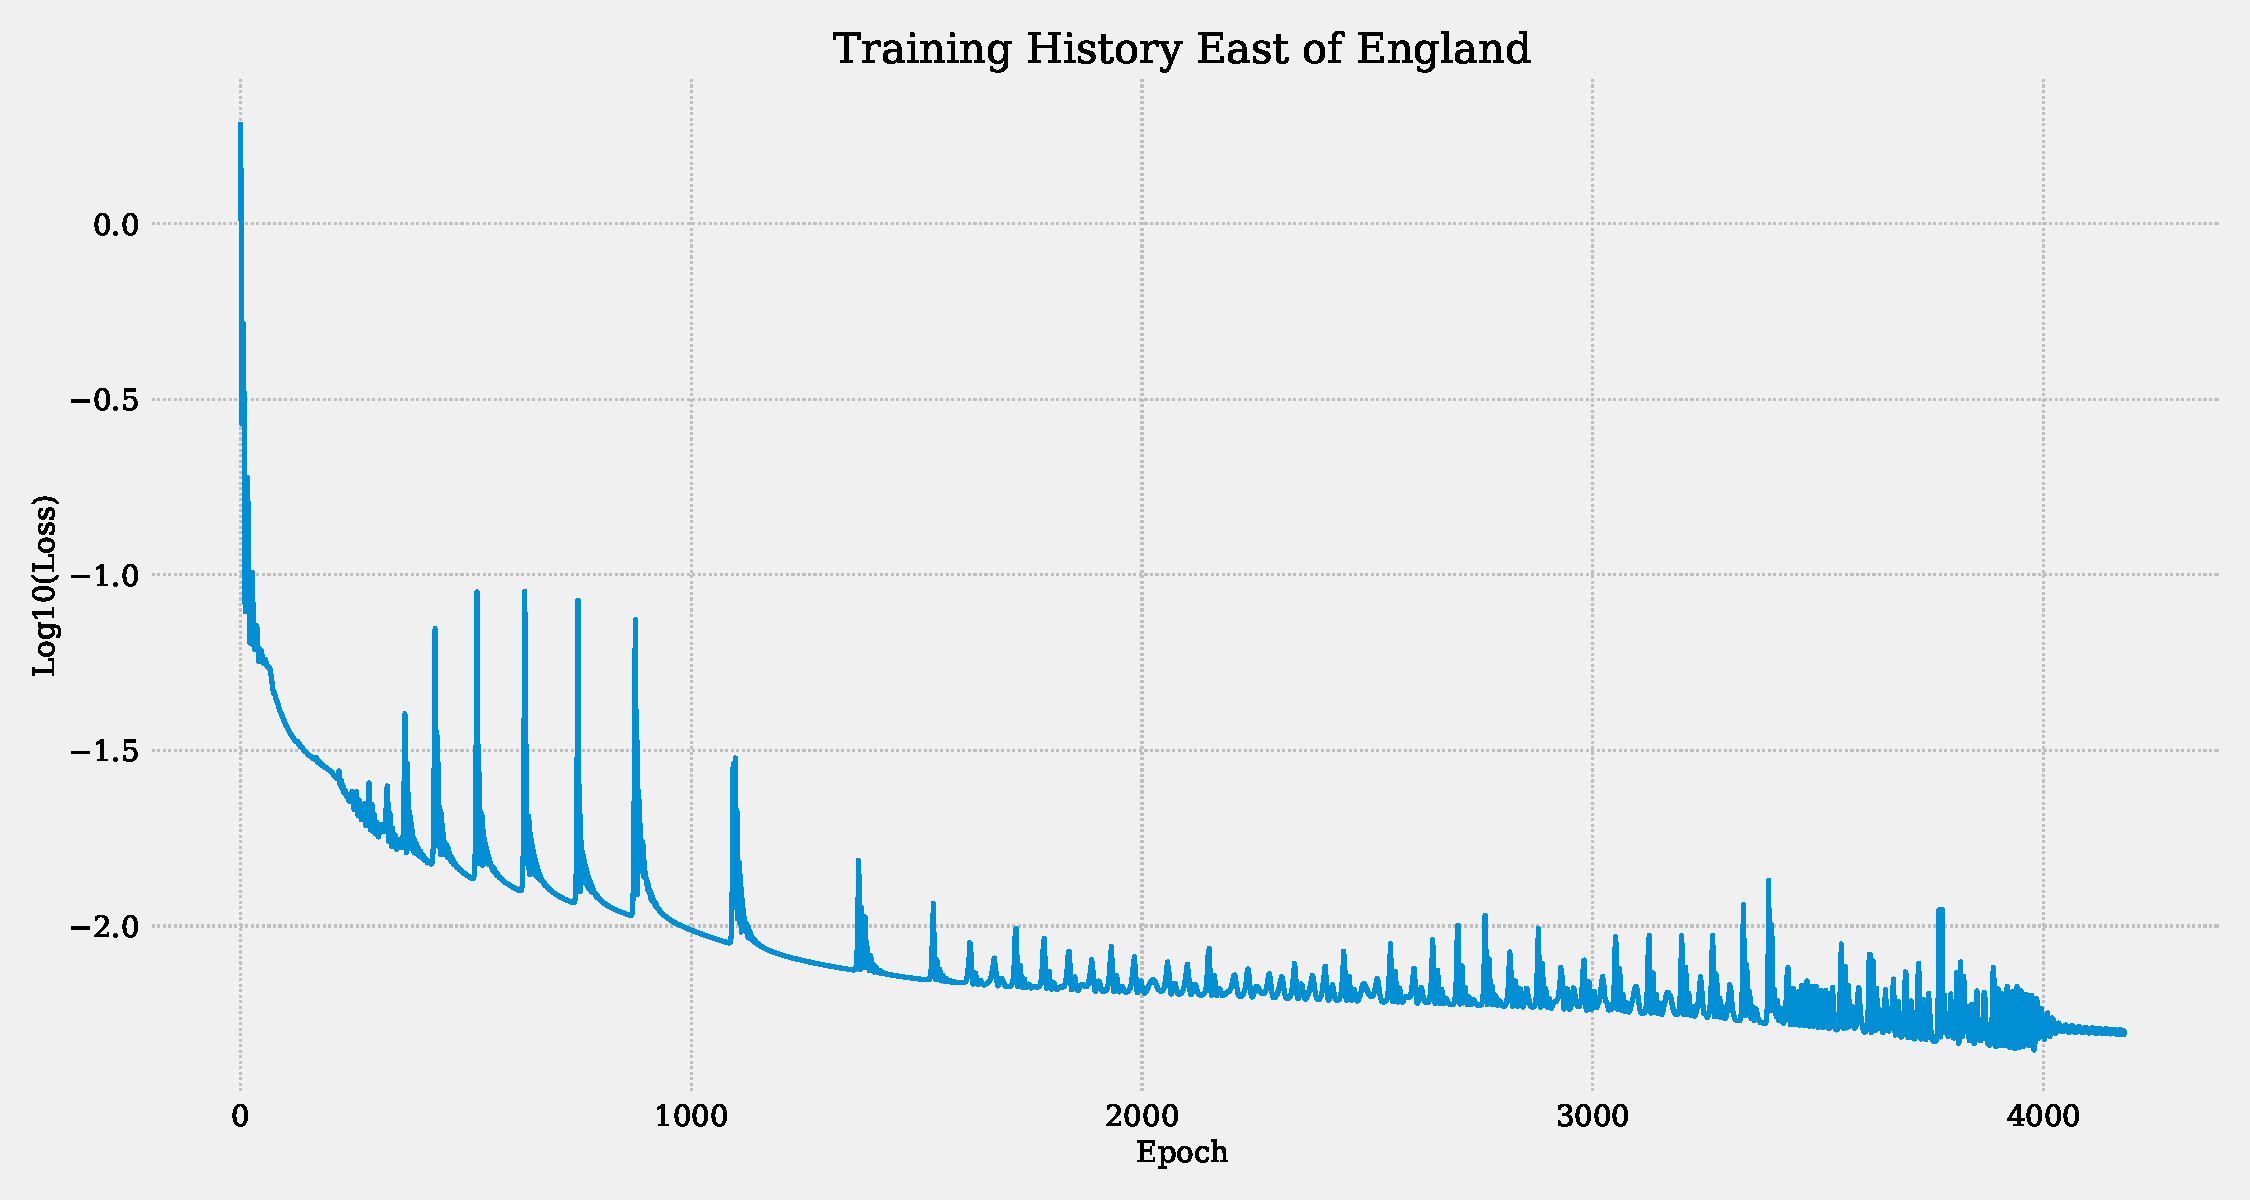
\includegraphics[width=0.8\textwidth]{images/pinn/Training_History_East of England.pdf}
    \caption{Training history of the PINN model for the East of England region.}
    \label{fig:Training_History_East_of_England}
\end{figure*}

\begin{figure*}[ht]
    \centering
    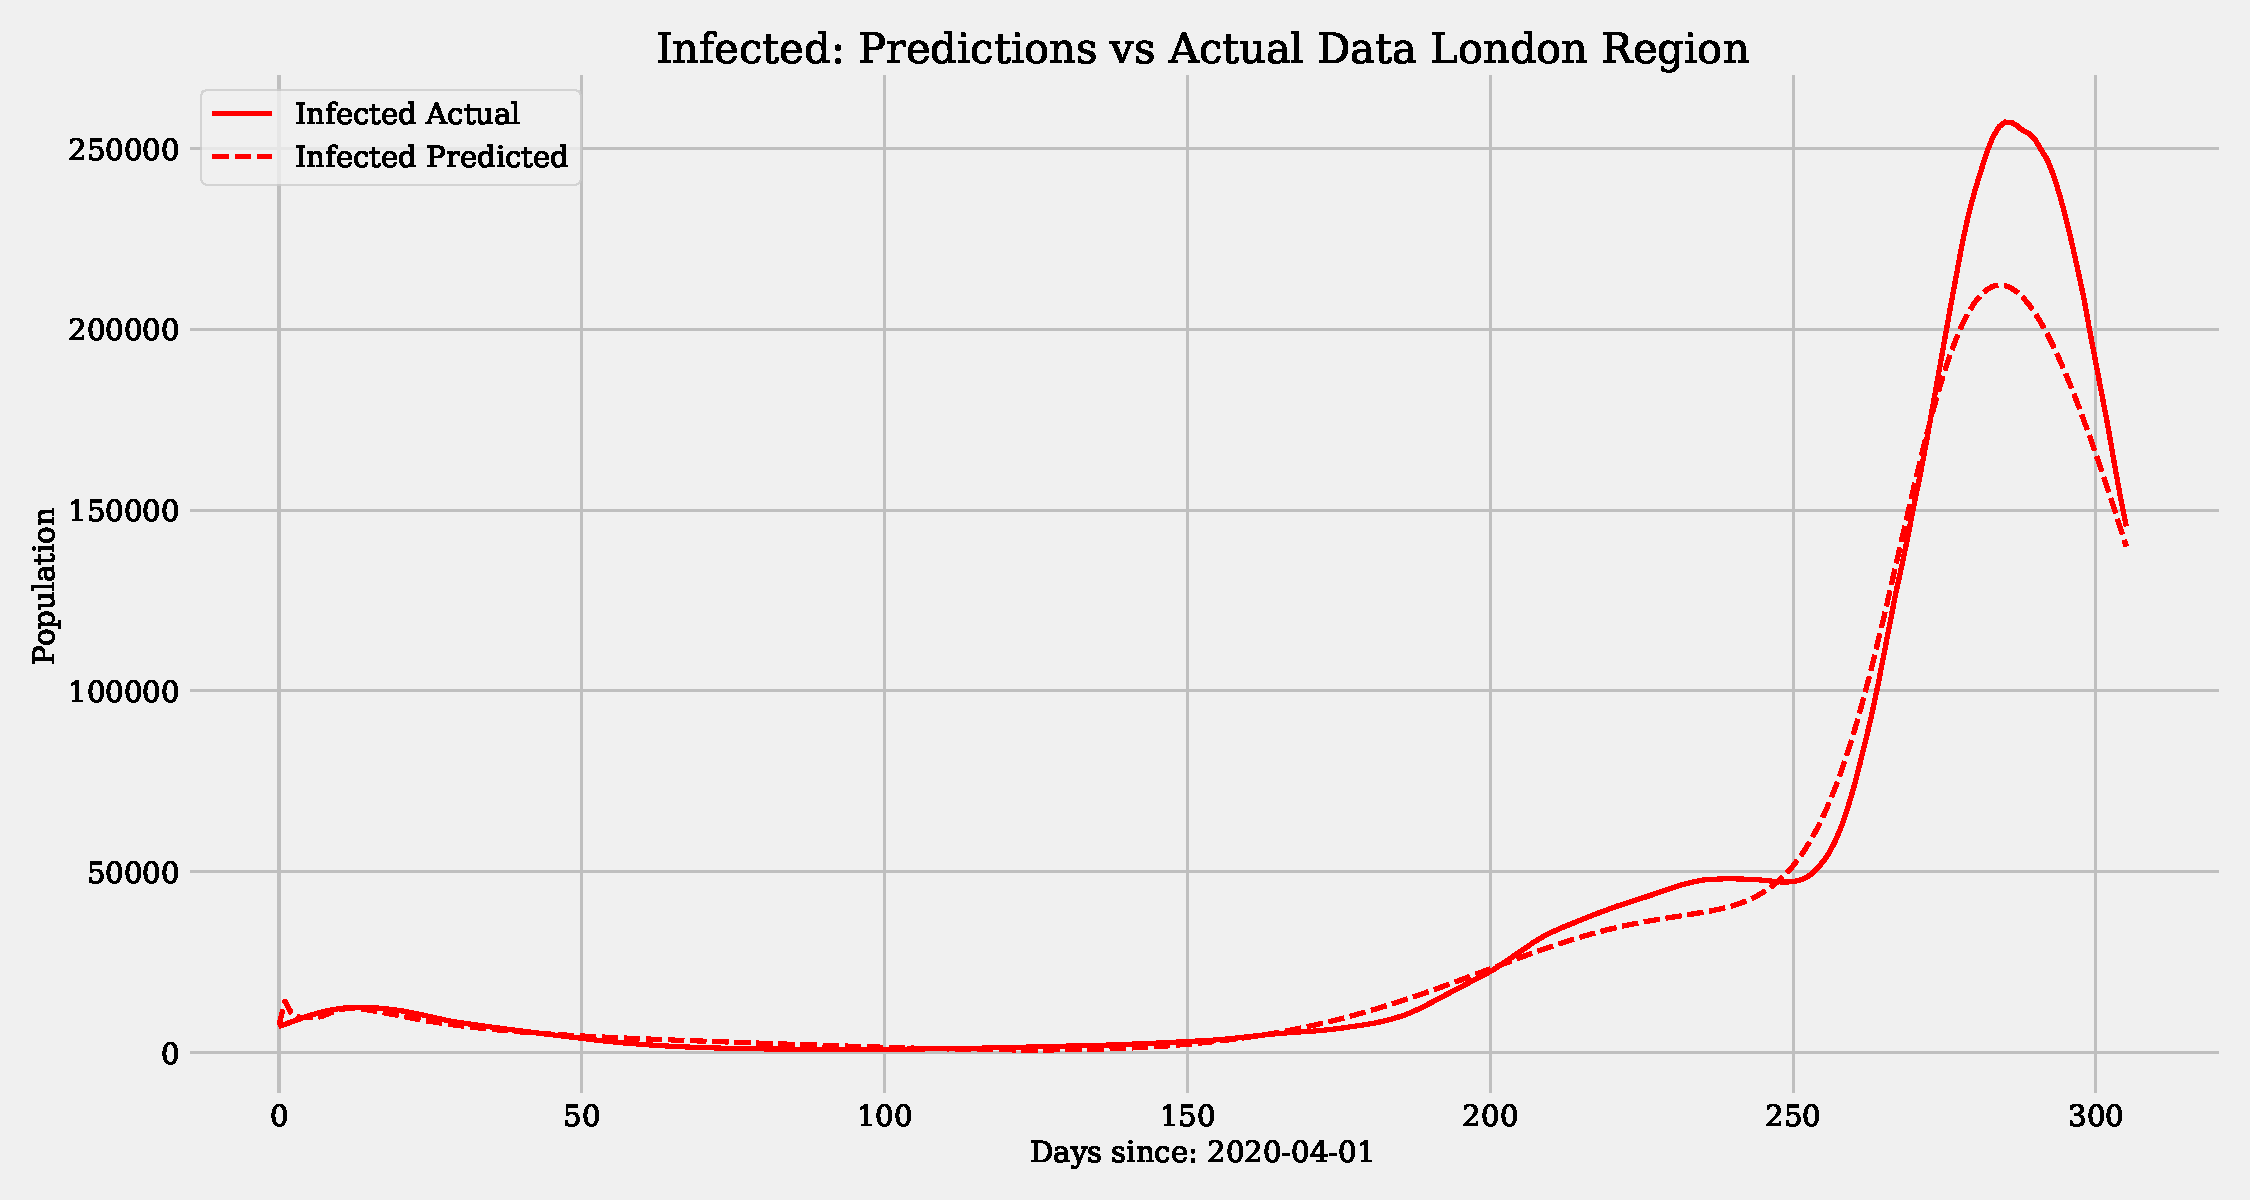
\includegraphics[width=0.8\textwidth]{images/pinn/I_predictions_London Region.pdf}
    \caption{Predicted number of infectious individuals in the London region.}
    \label{fig:I_predictions_London}
\end{figure*}

\begin{figure*}[ht]
    \centering
    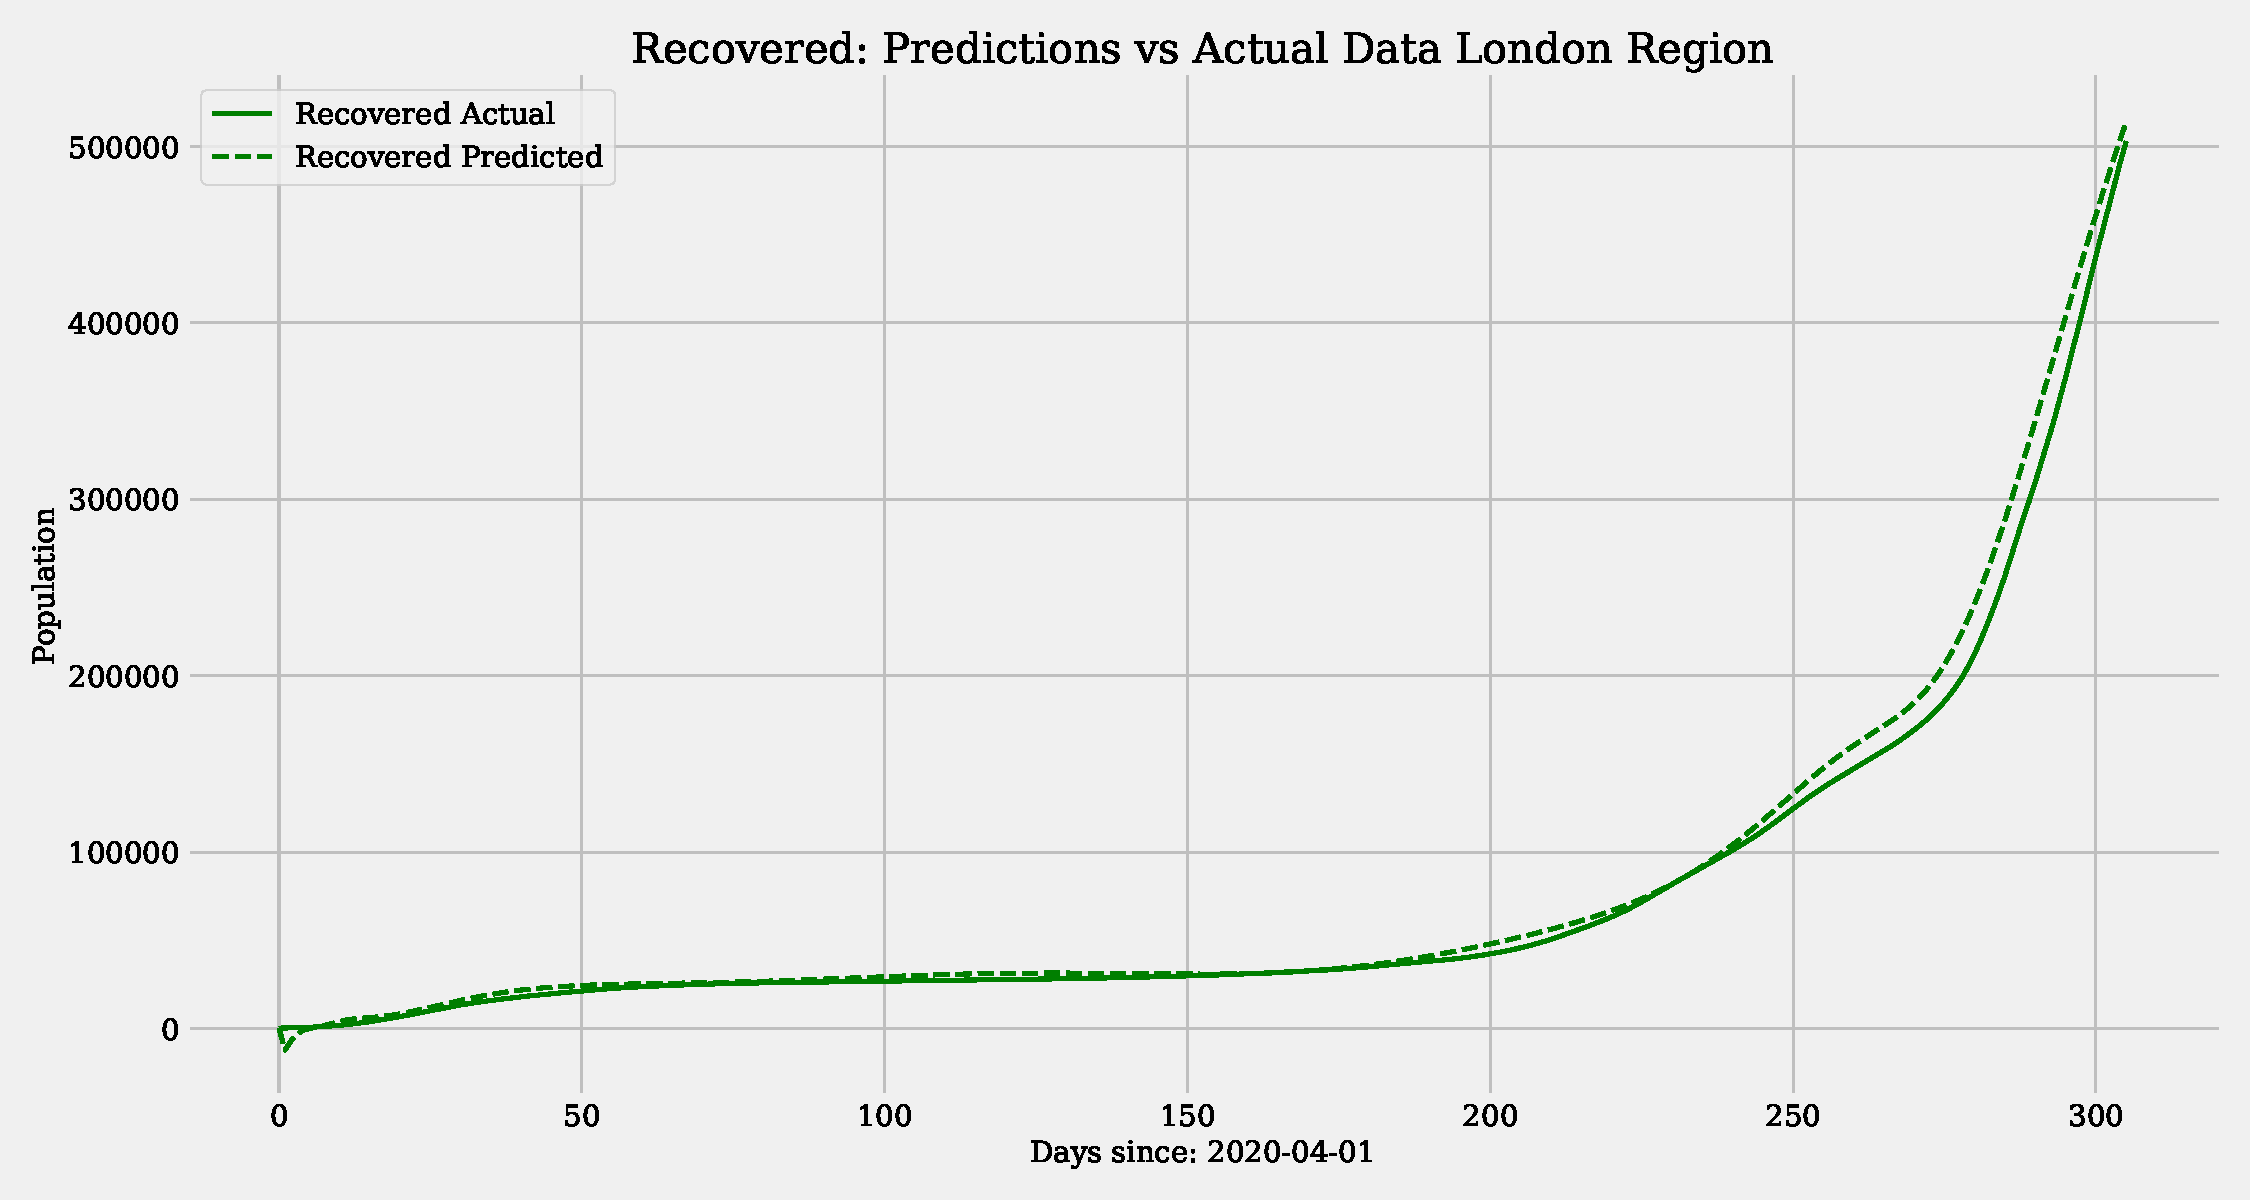
\includegraphics[width=0.8\textwidth]{images/pinn/R_predictions_London Region.pdf}
    \caption{Predicted number of recovered individuals in the London region.}
    \label{fig:R_predictions_London}
\end{figure*}

\begin{figure*}[ht]
    \centering
    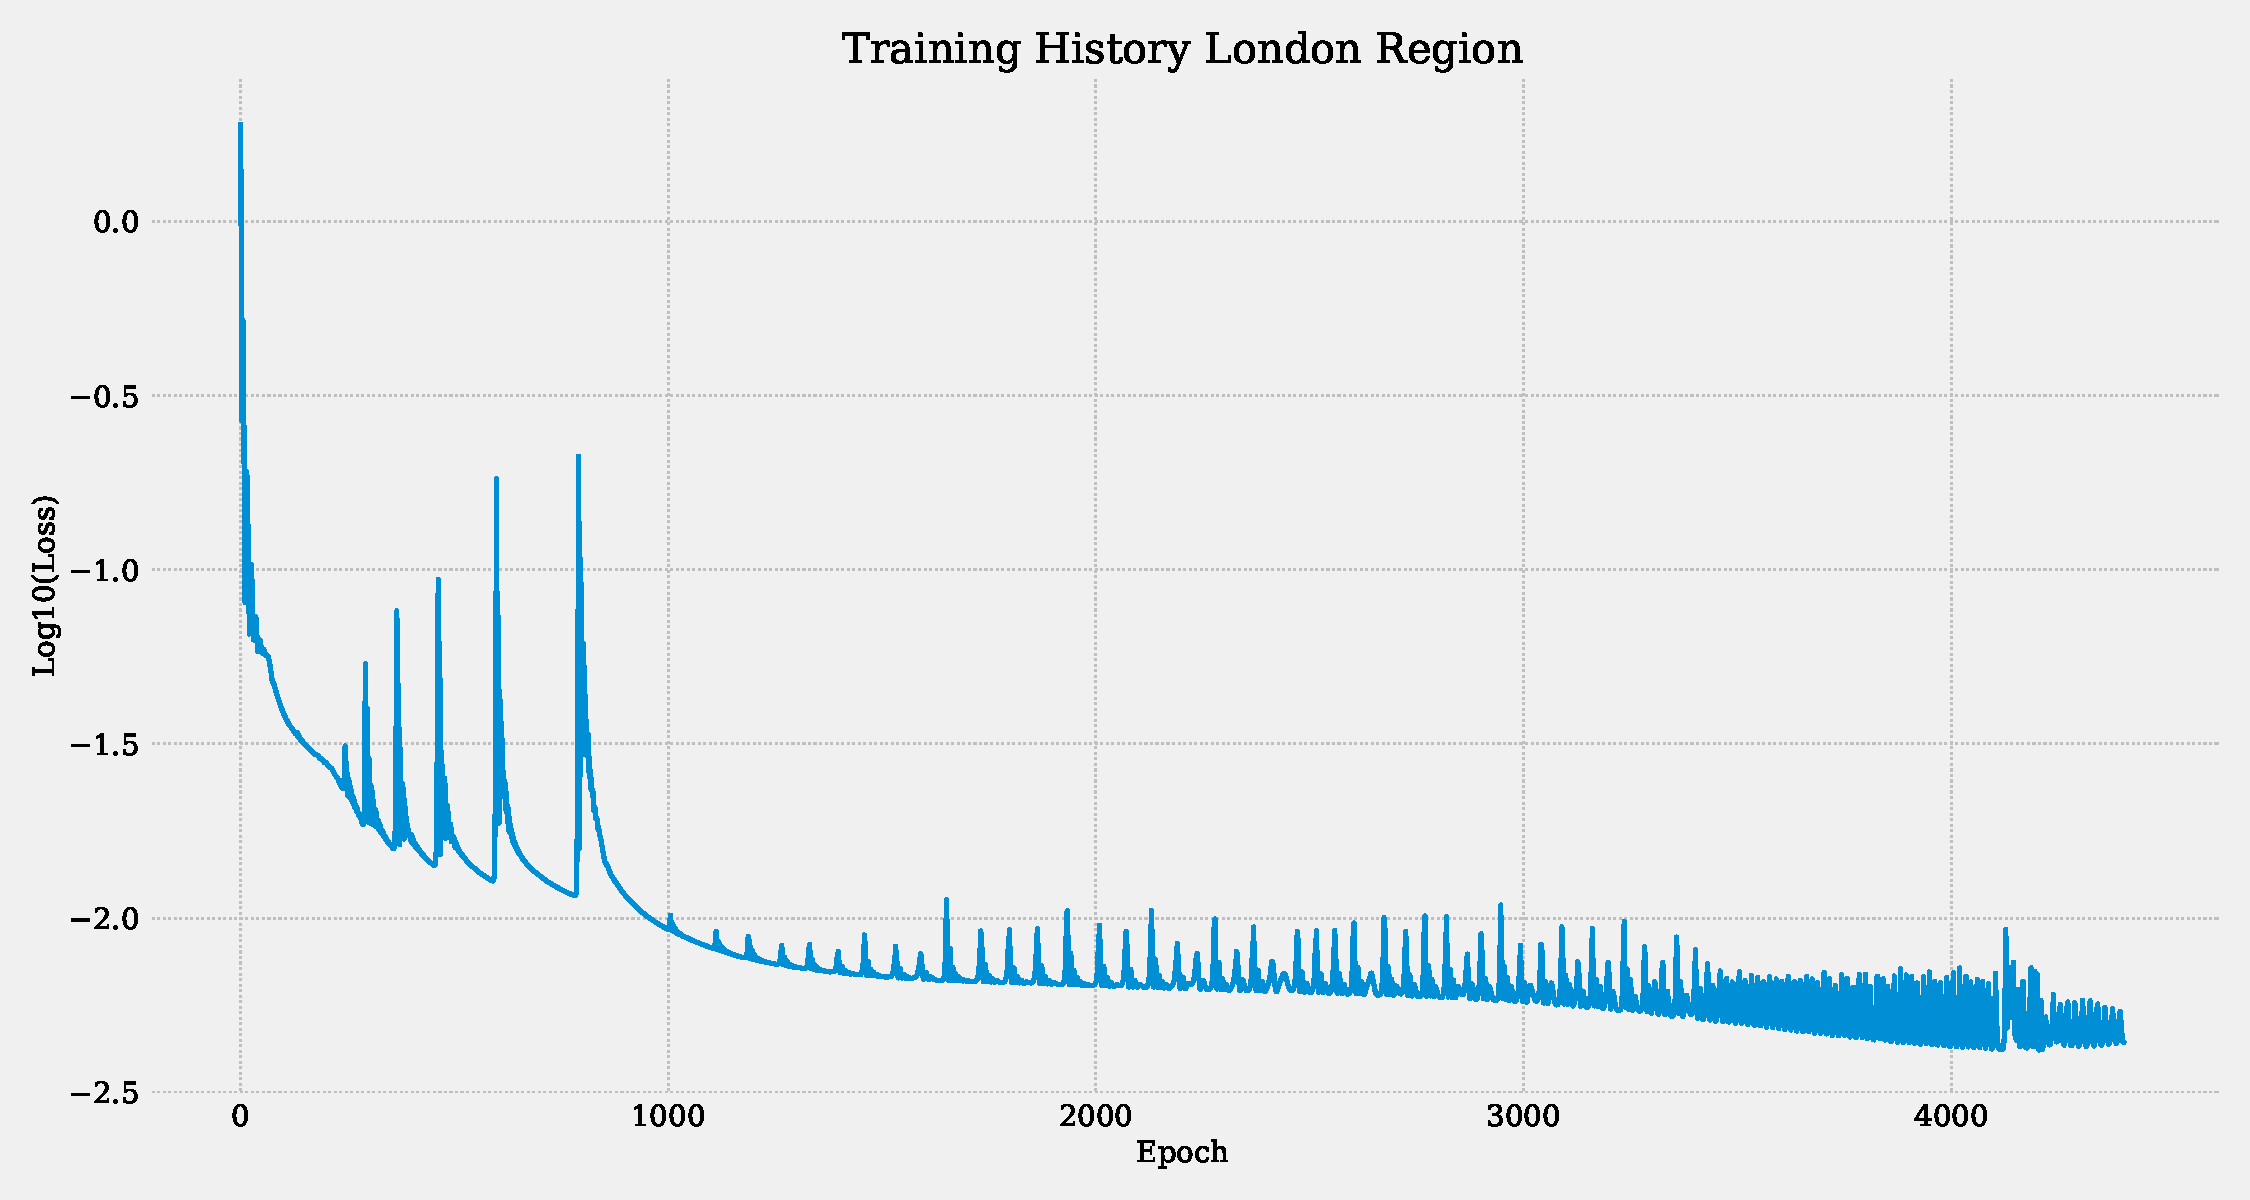
\includegraphics[width=0.8\textwidth]{images/pinn/Training_History_London Region.pdf}
    \caption{Training history of the PINN model for the London region.}
    \label{fig:Training_History_London}
\end{figure*}


\bibliographystyle{alphaurl}
\bibliography{refs}
\end{document}